\documentclass[a4paper,10pt,twoside]{report}

\usepackage{abstract}
\usepackage{graphicx}
\usepackage{placeins}
\usepackage{hyperref}
\usepackage{pdfpages}
\usepackage{fullpage}
\usepackage[bf]{caption}
\usepackage[english]{babel}
\usepackage{verbatim}
\usepackage{cite}
\usepackage{wrapfig}
\usepackage[marginpar]{todo}
\usepackage{paralist}
\usepackage{booktabs}
\usepackage{subcaption}
\usepackage{mathtools}
\usepackage{fancyhdr}
\usepackage{tikz}
\usepackage{gnuplot-lua-tikz}
\usetikzlibrary{calc,intersections}
\usepackage{amssymb}

\hypersetup{
    colorlinks,
    pdftitle={Evaluation Report Localization Option 1 IN4254 Smart Phone Sensing},
    pdfauthor={in4254-dhoepelman-mprovokluit},
}

\setlength{\parindent}{0pt}
\setlength{\parskip}{2ex}

\usepackage[utf8]{inputenc}

% Tex Live 2012 Qrazy Qwartel PPA for Preppy Pangolin:
% sudo apt-add-repository ppa:texlive-backports/ppa
% sudo apt-get update
% sudo apt-get install texlive texlive-latex-extra texlive-fonts-extra

% \usepackage{PTSans}
% \renewcommand*\familydefault{\sfdefault} %% Only if the base font of the document is to be sans serif
\usepackage[T1]{fontenc}

\newcommand{\axis}[1]{$#1$\nobreakdash-axis}
\newcommand{\plane}[2]{$#1#2$\nobreakdash-plane}

\title{\huge{\textbf{Evaluation Report\\Localization\\Option 1}\\IN4254 Smart Phone Sensing}}
\date{\today}
\author{David Hoepelman (1521969) \and Mark Provo Kluit (1263099)}

\setlength{\headheight}{15pt}
\addtolength{\headsep}{15pt} % no love between header and main text
%\addtolength{\textheight}{-20pt} % more space between text and empty footer

\pagestyle{fancy}
\renewcommand{\chaptermark}[1]{\markboth{Chapter\ \thechapter\ #1}{}}
\renewcommand{\sectionmark}[1]{\markright{\thesection\ #1}{}}
 
\fancyhf{}
\fancyhead[LE,RO]{\thepage}
\fancyhead[RE]{\textit{\nouppercase{\leftmark}}}
\fancyhead[LO]{\textit{\nouppercase{\rightmark}}}
 
\fancypagestyle{plain}{ %
\fancyhf{} % remove everything
\renewcommand{\headrulewidth}{0pt} % remove lines as well
\renewcommand{\footrulewidth}{0pt}}

\begin{document}

\maketitle

\newpage
\pagenumbering{roman}

%\phantomsection
\addcontentsline{toc}{chapter}{Preface}
\chapter*{Preface}
\label{sec:preface}
TODO


% 1: up to sections; 2: up to subsections
%\setcounter{tocdepth}{1}
%\tableofcontents

\newpage
\pagenumbering{arabic}

\setcounter{chapter}{1}
% Slide 20 of Lecture04.pdf

\section{Data Collection}
\label{sec:data-collections}

TODO

\section{Data Processing}
\label{sec:data-processing}

TODO

\section{Radio Map}
\label{sec:radio-map}

TODO

\section{Localization Method}
\label{sec:localization-method}

TODO

\section{Evaluation}
\label{sec:evaluation}

TODO

\section{Discussion}
\label{sec:disccusion}

TODO


\clearpage
\phantomsection
\addcontentsline{toc}{chapter}{Bibliography}
% styles: abbrv, ieeetr, plain
\bibliographystyle{abbrv}
\bibliography{report}

\newpage
\appendix

\chapter{Visualization Training Data}
\label{sec:app-visualization-training}

%\tikzset{global scale/.style={
%    scale=#1,
%    every node/.style={scale=#1}
%  }
%}

\begin{figure}[ht]
    \centering
%    \begin{tikzpicture}[gnuplot]
%% generated with GNUPLOT 4.7p0 (Lua 5.1; terminal rev. 99, script rev. 100)
%% 6-5-2014 20:00:55
\path (0.000,0.000) rectangle (12.500,8.750);
\gpcolor{color=gp lt color border}
\gpsetlinetype{gp lt border}
\gpsetlinewidth{1.00}
\draw[gp path] (1.437,2.277)--(3.750,4.137);
\draw[gp path] (7.755,3.063)--(3.750,4.137);
\draw[gp path] (1.437,2.277)--(1.437,5.995);
\draw[gp path] (1.437,2.277)--(1.534,2.355);
\node[gp node center] at (1.338,2.144) {-2};
\draw[gp path] (3.750,4.137)--(3.653,4.059);
\draw[gp path] (1.938,2.143)--(2.035,2.221);
\node[gp node center] at (1.839,2.010) {-1.5};
\draw[gp path] (4.251,4.002)--(4.154,3.924);
\draw[gp path] (2.438,2.009)--(2.535,2.087);
\node[gp node center] at (2.339,1.875) {-1};
\draw[gp path] (4.750,3.868)--(4.653,3.790);
\draw[gp path] (2.939,1.875)--(3.036,1.953);
\node[gp node center] at (2.840,1.741) {-0.5};
\draw[gp path] (5.251,3.734)--(5.154,3.656);
\draw[gp path] (3.440,1.740)--(3.537,1.818);
\node[gp node center] at (3.341,1.607) { 0};
\draw[gp path] (5.752,3.600)--(5.655,3.522);
\draw[gp path] (3.941,1.606)--(4.038,1.684);
\node[gp node center] at (3.842,1.473) { 0.5};
\draw[gp path] (6.253,3.466)--(6.156,3.388);
\draw[gp path] (4.442,1.472)--(4.539,1.550);
\node[gp node center] at (4.342,1.339) { 1};
\draw[gp path] (6.754,3.331)--(6.657,3.254);
\draw[gp path] (4.941,1.338)--(5.038,1.416);
\node[gp node center] at (4.842,1.205) { 1.5};
\draw[gp path] (7.254,3.197)--(7.157,3.119);
\draw[gp path] (5.442,1.204)--(5.539,1.282);
\node[gp node center] at (5.343,1.070) { 2};
\draw[gp path] (7.755,3.063)--(7.658,2.985);
\draw[gp path] (5.442,1.204)--(5.286,1.245);
\node[gp node center] at (5.601,1.132) {-3};
\draw[gp path] (1.437,2.277)--(1.593,2.235);
\draw[gp path] (5.699,1.410)--(5.543,1.452);
\node[gp node center] at (5.858,1.339) {-2.5};
\draw[gp path] (1.694,2.484)--(1.850,2.442);
\draw[gp path] (5.956,1.617)--(5.800,1.659);
\node[gp node center] at (6.115,1.545) {-2};
\draw[gp path] (1.951,2.690)--(2.107,2.649);
\draw[gp path] (6.213,1.824)--(6.057,1.865);
\node[gp node center] at (6.372,1.752) {-1.5};
\draw[gp path] (2.208,2.897)--(2.364,2.855);
\draw[gp path] (6.470,2.030)--(6.314,2.072);
\node[gp node center] at (6.629,1.959) {-1};
\draw[gp path] (2.465,3.104)--(2.621,3.062);
\draw[gp path] (6.727,2.237)--(6.571,2.278);
\node[gp node center] at (6.886,2.165) {-0.5};
\draw[gp path] (2.722,3.310)--(2.878,3.268);
\draw[gp path] (6.984,2.443)--(6.828,2.485);
\node[gp node center] at (7.143,2.372) { 0};
\draw[gp path] (2.979,3.517)--(3.135,3.475);
\draw[gp path] (7.241,2.650)--(7.085,2.692);
\node[gp node center] at (7.400,2.578) { 0.5};
\draw[gp path] (3.236,3.723)--(3.392,3.682);
\draw[gp path] (7.498,2.856)--(7.342,2.898);
\node[gp node center] at (7.657,2.785) { 1};
\draw[gp path] (3.493,3.930)--(3.649,3.888);
\draw[gp path] (7.755,3.063)--(7.599,3.105);
\node[gp node center] at (7.914,2.992) { 1.5};
\draw[gp path] (3.750,4.137)--(3.906,4.095);
\draw[gp path] (1.437,3.517)--(1.617,3.517);
\node[gp node right] at (1.077,3.517) {-0.5};
\draw[gp path] (1.437,3.930)--(1.617,3.930);
\node[gp node right] at (1.077,3.930) { 0};
\draw[gp path] (1.437,4.343)--(1.617,4.343);
\node[gp node right] at (1.077,4.343) { 0.5};
\draw[gp path] (1.437,4.755)--(1.617,4.755);
\node[gp node right] at (1.077,4.755) { 1};
\draw[gp path] (1.437,5.169)--(1.617,5.169);
\node[gp node right] at (1.077,5.169) { 1.5};
\draw[gp path] (1.437,5.582)--(1.617,5.582);
\node[gp node right] at (1.077,5.582) { 2};
\draw[gp path] (1.437,5.995)--(1.617,5.995);
\node[gp node right] at (1.077,5.995) { 2.5};
\node[gp node center] at (0.149,4.755) {MeanZ};
\node[gp node right] at (10.143,7.645) {Sitting};
\gpcolor{color=gp lt color 0}
\gpsetpointsize{4.00}
\gppoint{gp mark 1}{(4.980,4.632)}
\gppoint{gp mark 1}{(4.980,4.633)}
\gppoint{gp mark 1}{(4.981,4.633)}
\gppoint{gp mark 1}{(4.981,4.633)}
\gppoint{gp mark 1}{(4.981,4.633)}
\gppoint{gp mark 1}{(4.980,4.633)}
\gppoint{gp mark 1}{(4.981,4.634)}
\gppoint{gp mark 1}{(4.980,4.633)}
\gppoint{gp mark 1}{(4.980,4.632)}
\gppoint{gp mark 1}{(4.980,4.633)}
\gppoint{gp mark 1}{(4.981,4.633)}
\gppoint{gp mark 1}{(4.980,4.633)}
\gppoint{gp mark 1}{(4.979,4.633)}
\gppoint{gp mark 1}{(4.879,4.607)}
\gppoint{gp mark 1}{(4.811,4.549)}
\gppoint{gp mark 1}{(4.901,4.372)}
\gppoint{gp mark 1}{(4.792,4.623)}
\gppoint{gp mark 1}{(4.765,4.590)}
\gppoint{gp mark 1}{(4.741,4.547)}
\gppoint{gp mark 1}{(4.778,4.684)}
\gppoint{gp mark 1}{(4.654,4.556)}
\gppoint{gp mark 1}{(4.848,4.961)}
\gppoint{gp mark 1}{(4.634,4.627)}
\gppoint{gp mark 1}{(4.668,4.513)}
\gppoint{gp mark 1}{(4.444,4.690)}
\gppoint{gp mark 1}{(4.604,4.952)}
\gppoint{gp mark 1}{(4.665,5.671)}
\gppoint{gp mark 1}{(4.621,5.652)}
\gppoint{gp mark 1}{(4.608,5.571)}
\gppoint{gp mark 1}{(4.694,5.618)}
\gppoint{gp mark 1}{(4.679,5.546)}
\gppoint{gp mark 1}{(4.655,5.592)}
\gppoint{gp mark 1}{(4.579,5.590)}
\gppoint{gp mark 1}{(4.561,5.514)}
\gppoint{gp mark 1}{(4.571,5.536)}
\gppoint{gp mark 1}{(4.460,5.454)}
\gppoint{gp mark 1}{(4.447,5.381)}
\gppoint{gp mark 1}{(4.253,5.575)}
\gppoint{gp mark 1}{(4.243,5.580)}
\gppoint{gp mark 1}{(4.981,4.632)}
\gppoint{gp mark 1}{(4.981,4.632)}
\gppoint{gp mark 1}{(4.982,4.632)}
\gppoint{gp mark 1}{(4.981,4.631)}
\gppoint{gp mark 1}{(4.982,4.632)}
\gppoint{gp mark 1}{(4.982,4.634)}
\gppoint{gp mark 1}{(4.981,4.634)}
\gppoint{gp mark 1}{(4.981,4.632)}
\gppoint{gp mark 1}{(4.981,4.632)}
\gppoint{gp mark 1}{(4.982,4.633)}
\gppoint{gp mark 1}{(4.981,4.632)}
\gppoint{gp mark 1}{(4.981,4.633)}
\gppoint{gp mark 1}{(4.982,4.633)}
\gppoint{gp mark 1}{(4.981,4.632)}
\gppoint{gp mark 1}{(4.982,4.633)}
\gppoint{gp mark 1}{(4.982,4.633)}
\gppoint{gp mark 1}{(4.981,4.634)}
\gppoint{gp mark 1}{(4.981,4.632)}
\gppoint{gp mark 1}{(4.981,4.632)}
\gppoint{gp mark 1}{(4.981,4.633)}
\gppoint{gp mark 1}{(4.981,4.632)}
\gppoint{gp mark 1}{(4.981,4.632)}
\gppoint{gp mark 1}{(4.981,4.634)}
\gppoint{gp mark 1}{(4.981,4.633)}
\gppoint{gp mark 1}{(4.982,4.634)}
\gppoint{gp mark 1}{(4.980,4.629)}
\gppoint{gp mark 1}{(4.980,4.625)}
\gppoint{gp mark 1}{(4.978,4.623)}
\gppoint{gp mark 1}{(4.979,4.623)}
\gppoint{gp mark 1}{(4.978,4.623)}
\gppoint{gp mark 1}{(4.979,4.623)}
\gppoint{gp mark 1}{(4.979,4.623)}
\gppoint{gp mark 1}{(4.978,4.623)}
\gppoint{gp mark 1}{(4.978,4.624)}
\gppoint{gp mark 1}{(4.979,4.623)}
\gppoint{gp mark 1}{(4.979,4.623)}
\gppoint{gp mark 1}{(4.979,4.623)}
\gppoint{gp mark 1}{(4.979,4.623)}
\gppoint{gp mark 1}{(4.980,4.623)}
\gppoint{gp mark 1}{(4.979,4.623)}
\gppoint{gp mark 1}{(4.978,4.624)}
\gppoint{gp mark 1}{(4.980,4.623)}
\gppoint{gp mark 1}{(4.979,4.623)}
\gppoint{gp mark 1}{(4.980,4.622)}
\gppoint{gp mark 1}{(4.965,4.726)}
\gppoint{gp mark 1}{(4.980,4.620)}
\gppoint{gp mark 1}{(4.980,4.620)}
\gppoint{gp mark 1}{(4.804,4.430)}
\gppoint{gp mark 1}{(4.957,4.555)}
\gppoint{gp mark 1}{(4.985,4.624)}
\gppoint{gp mark 1}{(4.839,4.749)}
\gppoint{gp mark 1}{(4.819,4.567)}
\gppoint{gp mark 1}{(5.024,4.700)}
\gppoint{gp mark 1}{(5.090,4.657)}
\gppoint{gp mark 1}{(4.981,4.632)}
\gppoint{gp mark 1}{(4.982,4.632)}
\gppoint{gp mark 1}{(4.982,4.633)}
\gppoint{gp mark 1}{(4.982,4.631)}
\gppoint{gp mark 1}{(4.982,4.631)}
\gppoint{gp mark 1}{(4.981,4.632)}
\gppoint{gp mark 1}{(4.982,4.632)}
\gppoint{gp mark 1}{(4.981,4.632)}
\gppoint{gp mark 1}{(4.981,4.632)}
\gppoint{gp mark 1}{(4.981,4.631)}
\gppoint{gp mark 1}{(4.982,4.632)}
\gppoint{gp mark 1}{(4.981,4.631)}
\gppoint{gp mark 1}{(4.981,4.631)}
\gppoint{gp mark 1}{(4.982,4.633)}
\gppoint{gp mark 1}{(4.982,4.632)}
\gppoint{gp mark 1}{(4.982,4.631)}
\gppoint{gp mark 1}{(4.981,4.633)}
\gppoint{gp mark 1}{(10.785,7.645)}
\gpcolor{color=gp lt color border}
\node[gp node right] at (10.143,7.337) {Walking};
\gpcolor{color=gp lt color 1}
\gppoint{gp mark 2}{(4.830,4.603)}
\gppoint{gp mark 2}{(4.923,4.678)}
\gppoint{gp mark 2}{(4.993,4.726)}
\gppoint{gp mark 2}{(4.842,4.564)}
\gppoint{gp mark 2}{(4.946,4.576)}
\gppoint{gp mark 2}{(4.898,4.372)}
\gppoint{gp mark 2}{(4.943,4.645)}
\gppoint{gp mark 2}{(4.759,4.559)}
\gppoint{gp mark 2}{(4.936,4.618)}
\gppoint{gp mark 2}{(4.821,4.825)}
\gppoint{gp mark 2}{(4.822,4.616)}
\gppoint{gp mark 2}{(4.933,4.684)}
\gppoint{gp mark 2}{(4.735,4.524)}
\gppoint{gp mark 2}{(4.762,4.632)}
\gppoint{gp mark 2}{(4.914,4.646)}
\gppoint{gp mark 2}{(4.716,4.494)}
\gppoint{gp mark 2}{(4.772,4.556)}
\gppoint{gp mark 2}{(4.738,4.692)}
\gppoint{gp mark 2}{(4.938,4.588)}
\gppoint{gp mark 2}{(4.815,4.652)}
\gppoint{gp mark 2}{(4.867,4.669)}
\gppoint{gp mark 2}{(4.821,4.678)}
\gppoint{gp mark 2}{(4.846,4.659)}
\gppoint{gp mark 2}{(4.759,4.625)}
\gppoint{gp mark 2}{(4.804,4.607)}
\gppoint{gp mark 2}{(4.734,4.577)}
\gppoint{gp mark 2}{(4.853,4.561)}
\gppoint{gp mark 2}{(4.925,4.587)}
\gppoint{gp mark 2}{(4.803,4.683)}
\gppoint{gp mark 2}{(4.827,4.586)}
\gppoint{gp mark 2}{(4.696,4.662)}
\gppoint{gp mark 2}{(4.707,4.623)}
\gppoint{gp mark 2}{(4.674,4.501)}
\gppoint{gp mark 2}{(4.494,4.383)}
\gppoint{gp mark 2}{(4.938,4.907)}
\gppoint{gp mark 2}{(4.841,4.597)}
\gppoint{gp mark 2}{(4.776,4.662)}
\gppoint{gp mark 2}{(4.779,4.580)}
\gppoint{gp mark 2}{(4.753,4.701)}
\gppoint{gp mark 2}{(4.756,4.526)}
\gppoint{gp mark 2}{(5.393,6.150)}
\gppoint{gp mark 2}{(5.096,5.734)}
\gppoint{gp mark 2}{(4.825,4.805)}
\gppoint{gp mark 2}{(4.630,4.666)}
\gppoint{gp mark 2}{(4.877,5.789)}
\gppoint{gp mark 2}{(4.667,4.904)}
\gppoint{gp mark 2}{(4.534,4.722)}
\gppoint{gp mark 2}{(4.752,5.485)}
\gppoint{gp mark 2}{(4.857,5.409)}
\gppoint{gp mark 2}{(5.087,6.087)}
\gppoint{gp mark 2}{(4.800,5.453)}
\gppoint{gp mark 2}{(4.818,5.551)}
\gppoint{gp mark 2}{(4.705,5.321)}
\gppoint{gp mark 2}{(4.627,4.708)}
\gppoint{gp mark 2}{(4.920,5.634)}
\gppoint{gp mark 2}{(4.687,5.499)}
\gppoint{gp mark 2}{(4.449,4.750)}
\gppoint{gp mark 2}{(4.747,5.581)}
\gppoint{gp mark 2}{(4.596,5.886)}
\gppoint{gp mark 2}{(4.617,5.605)}
\gppoint{gp mark 2}{(4.669,5.994)}
\gppoint{gp mark 2}{(4.658,5.717)}
\gppoint{gp mark 2}{(4.564,5.430)}
\gppoint{gp mark 2}{(4.197,4.699)}
\gppoint{gp mark 2}{(4.536,5.922)}
\gppoint{gp mark 2}{(4.462,6.154)}
\gppoint{gp mark 2}{(4.426,5.726)}
\gppoint{gp mark 2}{(4.263,5.467)}
\gppoint{gp mark 2}{(4.076,5.295)}
\gppoint{gp mark 2}{(4.895,4.694)}
\gppoint{gp mark 2}{(4.990,4.494)}
\gppoint{gp mark 2}{(4.794,4.642)}
\gppoint{gp mark 2}{(4.879,4.561)}
\gppoint{gp mark 2}{(4.902,4.623)}
\gppoint{gp mark 2}{(4.889,4.557)}
\gppoint{gp mark 2}{(4.956,4.605)}
\gppoint{gp mark 2}{(4.870,4.604)}
\gppoint{gp mark 2}{(4.905,4.620)}
\gppoint{gp mark 2}{(4.942,4.576)}
\gppoint{gp mark 2}{(4.882,4.557)}
\gppoint{gp mark 2}{(5.010,4.485)}
\gppoint{gp mark 2}{(4.934,4.678)}
\gppoint{gp mark 2}{(5.018,4.505)}
\gppoint{gp mark 2}{(4.863,4.497)}
\gppoint{gp mark 2}{(5.600,6.484)}
\gppoint{gp mark 2}{(5.084,4.706)}
\gppoint{gp mark 2}{(5.050,4.492)}
\gppoint{gp mark 2}{(4.831,4.546)}
\gppoint{gp mark 2}{(5.125,4.613)}
\gppoint{gp mark 2}{(5.129,4.664)}
\gppoint{gp mark 2}{(4.960,4.568)}
\gppoint{gp mark 2}{(5.009,4.740)}
\gppoint{gp mark 2}{(4.793,4.700)}
\gppoint{gp mark 2}{(4.949,4.606)}
\gppoint{gp mark 2}{(5.076,4.721)}
\gppoint{gp mark 2}{(4.982,4.638)}
\gppoint{gp mark 2}{(5.065,4.558)}
\gppoint{gp mark 2}{(5.057,4.614)}
\gppoint{gp mark 2}{(5.023,4.570)}
\gppoint{gp mark 2}{(5.195,4.503)}
\gppoint{gp mark 2}{(5.198,4.509)}
\gppoint{gp mark 2}{(5.111,4.444)}
\gppoint{gp mark 2}{(5.063,4.448)}
\gppoint{gp mark 2}{(4.941,4.369)}
\gppoint{gp mark 2}{(5.233,4.249)}
\gppoint{gp mark 2}{(5.065,4.290)}
\gppoint{gp mark 2}{(5.260,4.458)}
\gppoint{gp mark 2}{(5.520,4.614)}
\gppoint{gp mark 2}{(5.727,4.401)}
\gppoint{gp mark 2}{(4.853,4.550)}
\gppoint{gp mark 2}{(10.785,7.337)}
\gpcolor{color=gp lt color border}
\node[gp node right] at (10.143,7.029) {Running};
\gpcolor{color=gp lt color 2}
\gppoint{gp mark 3}{(4.683,5.211)}
\gppoint{gp mark 3}{(4.639,4.978)}
\gppoint{gp mark 3}{(4.606,4.857)}
\gppoint{gp mark 3}{(4.537,5.152)}
\gppoint{gp mark 3}{(4.491,5.211)}
\gppoint{gp mark 3}{(4.491,5.211)}
\gppoint{gp mark 3}{(4.599,4.614)}
\gppoint{gp mark 3}{(4.445,4.943)}
\gppoint{gp mark 3}{(4.538,4.590)}
\gppoint{gp mark 3}{(4.843,4.999)}
\gppoint{gp mark 3}{(4.368,5.172)}
\gppoint{gp mark 3}{(4.618,5.176)}
\gppoint{gp mark 3}{(4.558,5.064)}
\gppoint{gp mark 3}{(4.516,5.043)}
\gppoint{gp mark 3}{(4.208,5.071)}
\gppoint{gp mark 3}{(4.564,4.839)}
\gppoint{gp mark 3}{(5.058,5.236)}
\gppoint{gp mark 3}{(4.475,5.270)}
\gppoint{gp mark 3}{(4.392,5.317)}
\gppoint{gp mark 3}{(4.496,4.740)}
\gppoint{gp mark 3}{(4.046,5.752)}
\gppoint{gp mark 3}{(4.442,5.541)}
\gppoint{gp mark 3}{(4.525,4.805)}
\gppoint{gp mark 3}{(4.572,5.493)}
\gppoint{gp mark 3}{(4.424,5.027)}
\gppoint{gp mark 3}{(4.336,4.804)}
\gppoint{gp mark 3}{(4.401,4.740)}
\gppoint{gp mark 3}{(4.317,4.772)}
\gppoint{gp mark 3}{(3.939,5.695)}
\gppoint{gp mark 3}{(4.395,4.958)}
\gppoint{gp mark 3}{(4.271,5.572)}
\gppoint{gp mark 3}{(4.875,4.996)}
\gppoint{gp mark 3}{(3.990,5.711)}
\gppoint{gp mark 3}{(4.206,4.860)}
\gppoint{gp mark 3}{(4.429,5.230)}
\gppoint{gp mark 3}{(3.632,5.942)}
\gppoint{gp mark 3}{(4.190,5.750)}
\gppoint{gp mark 3}{(4.486,5.114)}
\gppoint{gp mark 3}{(4.486,5.114)}
\gppoint{gp mark 3}{(4.092,5.060)}
\gppoint{gp mark 3}{(3.823,5.000)}
\gppoint{gp mark 3}{(3.593,6.001)}
\gppoint{gp mark 3}{(4.322,5.287)}
\gppoint{gp mark 3}{(3.511,5.949)}
\gppoint{gp mark 3}{(4.111,5.409)}
\gppoint{gp mark 3}{(4.100,5.463)}
\gppoint{gp mark 3}{(4.165,5.456)}
\gppoint{gp mark 3}{(3.886,5.276)}
\gppoint{gp mark 3}{(3.919,5.606)}
\gppoint{gp mark 3}{(3.479,5.705)}
\gppoint{gp mark 3}{(4.503,5.145)}
\gppoint{gp mark 3}{(3.711,5.289)}
\gppoint{gp mark 3}{(4.098,4.828)}
\gppoint{gp mark 3}{(4.297,5.331)}
\gppoint{gp mark 3}{(3.027,5.602)}
\gppoint{gp mark 3}{(4.123,5.949)}
\gppoint{gp mark 3}{(4.406,5.699)}
\gppoint{gp mark 3}{(4.168,5.645)}
\gppoint{gp mark 3}{(4.210,5.844)}
\gppoint{gp mark 3}{(4.103,5.708)}
\gppoint{gp mark 3}{(4.141,5.754)}
\gppoint{gp mark 3}{(4.232,5.829)}
\gppoint{gp mark 3}{(3.921,5.540)}
\gppoint{gp mark 3}{(4.202,6.546)}
\gppoint{gp mark 3}{(3.986,5.699)}
\gppoint{gp mark 3}{(4.309,6.538)}
\gppoint{gp mark 3}{(3.962,5.945)}
\gppoint{gp mark 3}{(3.954,6.092)}
\gppoint{gp mark 3}{(3.926,5.924)}
\gppoint{gp mark 3}{(3.802,5.520)}
\gppoint{gp mark 3}{(3.927,5.769)}
\gppoint{gp mark 3}{(3.798,5.970)}
\gppoint{gp mark 3}{(4.049,6.841)}
\gppoint{gp mark 3}{(3.571,5.976)}
\gppoint{gp mark 3}{(3.775,6.755)}
\gppoint{gp mark 3}{(3.572,6.280)}
\gppoint{gp mark 3}{(3.777,6.052)}
\gppoint{gp mark 3}{(3.793,6.389)}
\gppoint{gp mark 3}{(3.545,6.608)}
\gppoint{gp mark 3}{(3.745,7.010)}
\gppoint{gp mark 3}{(3.482,7.372)}
\gppoint{gp mark 3}{(4.672,5.337)}
\gppoint{gp mark 3}{(4.853,4.656)}
\gppoint{gp mark 3}{(4.854,4.935)}
\gppoint{gp mark 3}{(5.254,5.167)}
\gppoint{gp mark 3}{(4.604,4.422)}
\gppoint{gp mark 3}{(4.722,4.711)}
\gppoint{gp mark 3}{(4.931,5.345)}
\gppoint{gp mark 3}{(5.114,4.715)}
\gppoint{gp mark 3}{(4.987,5.009)}
\gppoint{gp mark 3}{(4.914,4.927)}
\gppoint{gp mark 3}{(4.990,4.665)}
\gppoint{gp mark 3}{(4.931,5.261)}
\gppoint{gp mark 3}{(5.056,5.658)}
\gppoint{gp mark 3}{(4.931,5.261)}
\gppoint{gp mark 3}{(4.838,5.190)}
\gppoint{gp mark 3}{(6.027,5.086)}
\gppoint{gp mark 3}{(5.063,5.553)}
\gppoint{gp mark 3}{(4.999,5.505)}
\gppoint{gp mark 3}{(5.161,6.054)}
\gppoint{gp mark 3}{(4.730,5.418)}
\gppoint{gp mark 3}{(5.141,5.033)}
\gppoint{gp mark 3}{(4.494,4.269)}
\gppoint{gp mark 3}{(5.465,4.696)}
\gppoint{gp mark 3}{(5.325,4.896)}
\gppoint{gp mark 3}{(5.211,5.194)}
\gppoint{gp mark 3}{(5.461,4.807)}
\gppoint{gp mark 3}{(5.670,5.023)}
\gppoint{gp mark 3}{(5.594,4.964)}
\gppoint{gp mark 3}{(5.949,4.488)}
\gppoint{gp mark 3}{(10.785,7.029)}
\gpcolor{color=gp lt color border}
\node[gp node right] at (10.143,6.721) {Stairs_Down};
\gpcolor{color=gp lt color 3}
\gppoint{gp mark 4}{(4.858,4.526)}
\gppoint{gp mark 4}{(5.185,5.257)}
\gppoint{gp mark 4}{(5.274,5.342)}
\gppoint{gp mark 4}{(5.147,5.194)}
\gppoint{gp mark 4}{(5.150,5.428)}
\gppoint{gp mark 4}{(4.955,4.855)}
\gppoint{gp mark 4}{(4.936,4.894)}
\gppoint{gp mark 4}{(4.961,4.828)}
\gppoint{gp mark 4}{(4.661,4.401)}
\gppoint{gp mark 4}{(5.120,5.315)}
\gppoint{gp mark 4}{(5.159,5.076)}
\gppoint{gp mark 4}{(5.115,5.320)}
\gppoint{gp mark 4}{(5.147,5.296)}
\gppoint{gp mark 4}{(4.711,4.656)}
\gppoint{gp mark 4}{(4.993,5.110)}
\gppoint{gp mark 4}{(5.148,5.436)}
\gppoint{gp mark 4}{(4.846,4.556)}
\gppoint{gp mark 4}{(4.556,4.751)}
\gppoint{gp mark 4}{(4.765,5.139)}
\gppoint{gp mark 4}{(4.658,4.707)}
\gppoint{gp mark 4}{(4.395,4.725)}
\gppoint{gp mark 4}{(5.184,5.323)}
\gppoint{gp mark 4}{(4.835,4.554)}
\gppoint{gp mark 4}{(5.158,4.944)}
\gppoint{gp mark 4}{(5.211,5.392)}
\gppoint{gp mark 4}{(5.166,5.225)}
\gppoint{gp mark 4}{(4.739,4.615)}
\gppoint{gp mark 4}{(5.095,4.684)}
\gppoint{gp mark 4}{(5.291,5.381)}
\gppoint{gp mark 4}{(5.311,5.413)}
\gppoint{gp mark 4}{(5.015,4.595)}
\gppoint{gp mark 4}{(5.036,4.699)}
\gppoint{gp mark 4}{(5.224,5.342)}
\gppoint{gp mark 4}{(4.815,4.538)}
\gppoint{gp mark 4}{(5.258,5.003)}
\gppoint{gp mark 4}{(4.822,4.710)}
\gppoint{gp mark 4}{(4.908,4.581)}
\gppoint{gp mark 4}{(5.012,4.619)}
\gppoint{gp mark 4}{(5.256,5.157)}
\gppoint{gp mark 4}{(5.152,4.547)}
\gppoint{gp mark 4}{(5.203,5.101)}
\gppoint{gp mark 4}{(5.238,4.770)}
\gppoint{gp mark 4}{(4.751,4.391)}
\gppoint{gp mark 4}{(4.763,4.532)}
\gppoint{gp mark 4}{(4.814,4.562)}
\gppoint{gp mark 4}{(5.336,5.147)}
\gppoint{gp mark 4}{(5.295,5.150)}
\gppoint{gp mark 4}{(5.260,4.995)}
\gppoint{gp mark 4}{(5.304,5.300)}
\gppoint{gp mark 4}{(4.997,4.540)}
\gppoint{gp mark 4}{(4.964,4.835)}
\gppoint{gp mark 4}{(5.398,5.283)}
\gppoint{gp mark 4}{(5.100,4.731)}
\gppoint{gp mark 4}{(4.891,4.554)}
\gppoint{gp mark 4}{(5.404,5.139)}
\gppoint{gp mark 4}{(5.258,5.135)}
\gppoint{gp mark 4}{(5.082,4.624)}
\gppoint{gp mark 4}{(4.888,4.363)}
\gppoint{gp mark 4}{(5.209,4.669)}
\gppoint{gp mark 4}{(5.375,5.112)}
\gppoint{gp mark 4}{(5.275,4.941)}
\gppoint{gp mark 4}{(5.410,5.003)}
\gppoint{gp mark 4}{(5.050,4.620)}
\gppoint{gp mark 4}{(5.380,5.204)}
\gppoint{gp mark 4}{(5.358,5.358)}
\gppoint{gp mark 4}{(5.366,4.970)}
\gppoint{gp mark 4}{(5.023,4.327)}
\gppoint{gp mark 4}{(5.321,5.038)}
\gppoint{gp mark 4}{(4.776,4.300)}
\gppoint{gp mark 4}{(4.961,4.657)}
\gppoint{gp mark 4}{(5.302,5.140)}
\gppoint{gp mark 4}{(4.925,4.354)}
\gppoint{gp mark 4}{(5.025,4.803)}
\gppoint{gp mark 4}{(5.554,5.397)}
\gppoint{gp mark 4}{(5.020,4.660)}
\gppoint{gp mark 4}{(5.379,4.896)}
\gppoint{gp mark 4}{(5.317,5.159)}
\gppoint{gp mark 4}{(5.539,5.208)}
\gppoint{gp mark 4}{(5.021,4.559)}
\gppoint{gp mark 4}{(5.189,4.568)}
\gppoint{gp mark 4}{(5.163,4.563)}
\gppoint{gp mark 4}{(5.533,5.144)}
\gppoint{gp mark 4}{(5.312,4.737)}
\gppoint{gp mark 4}{(5.101,4.558)}
\gppoint{gp mark 4}{(5.471,5.006)}
\gppoint{gp mark 4}{(5.113,4.505)}
\gppoint{gp mark 4}{(5.185,4.656)}
\gppoint{gp mark 4}{(5.055,4.463)}
\gppoint{gp mark 4}{(5.180,4.499)}
\gppoint{gp mark 4}{(5.091,4.511)}
\gppoint{gp mark 4}{(5.109,4.319)}
\gppoint{gp mark 4}{(5.294,4.476)}
\gppoint{gp mark 4}{(5.693,5.574)}
\gppoint{gp mark 4}{(5.530,4.978)}
\gppoint{gp mark 4}{(5.078,4.669)}
\gppoint{gp mark 4}{(5.433,4.834)}
\gppoint{gp mark 4}{(5.715,5.138)}
\gppoint{gp mark 4}{(5.363,4.703)}
\gppoint{gp mark 4}{(5.272,4.519)}
\gppoint{gp mark 4}{(5.327,4.668)}
\gppoint{gp mark 4}{(5.197,4.503)}
\gppoint{gp mark 4}{(5.300,4.327)}
\gppoint{gp mark 4}{(5.354,4.490)}
\gppoint{gp mark 4}{(5.364,4.393)}
\gppoint{gp mark 4}{(5.510,4.494)}
\gppoint{gp mark 4}{(5.345,4.363)}
\gppoint{gp mark 4}{(5.361,4.448)}
\gppoint{gp mark 4}{(5.516,4.439)}
\gppoint{gp mark 4}{(5.421,4.411)}
\gppoint{gp mark 4}{(5.518,4.272)}
\gppoint{gp mark 4}{(10.785,6.721)}
\gpcolor{color=gp lt color border}
\node[gp node right] at (10.143,6.413) {Stairs_Up};
\gpcolor{color=gp lt color 4}
\gppoint{gp mark 5}{(5.166,5.213)}
\gppoint{gp mark 5}{(4.846,4.681)}
\gppoint{gp mark 5}{(5.098,5.018)}
\gppoint{gp mark 5}{(4.802,4.597)}
\gppoint{gp mark 5}{(5.134,5.274)}
\gppoint{gp mark 5}{(5.001,4.630)}
\gppoint{gp mark 5}{(5.015,4.896)}
\gppoint{gp mark 5}{(5.134,5.034)}
\gppoint{gp mark 5}{(5.017,4.980)}
\gppoint{gp mark 5}{(4.847,4.646)}
\gppoint{gp mark 5}{(4.747,4.727)}
\gppoint{gp mark 5}{(4.752,4.614)}
\gppoint{gp mark 5}{(4.976,4.864)}
\gppoint{gp mark 5}{(5.038,4.830)}
\gppoint{gp mark 5}{(4.979,4.956)}
\gppoint{gp mark 5}{(4.769,4.550)}
\gppoint{gp mark 5}{(4.885,4.676)}
\gppoint{gp mark 5}{(4.989,4.838)}
\gppoint{gp mark 5}{(4.956,4.810)}
\gppoint{gp mark 5}{(4.873,4.655)}
\gppoint{gp mark 5}{(4.745,4.640)}
\gppoint{gp mark 5}{(4.912,4.876)}
\gppoint{gp mark 5}{(4.805,4.691)}
\gppoint{gp mark 5}{(4.867,4.710)}
\gppoint{gp mark 5}{(4.748,4.757)}
\gppoint{gp mark 5}{(4.785,4.584)}
\gppoint{gp mark 5}{(4.873,4.714)}
\gppoint{gp mark 5}{(4.745,4.702)}
\gppoint{gp mark 5}{(4.947,5.039)}
\gppoint{gp mark 5}{(4.772,4.705)}
\gppoint{gp mark 5}{(4.843,5.102)}
\gppoint{gp mark 5}{(4.733,4.777)}
\gppoint{gp mark 5}{(4.928,5.039)}
\gppoint{gp mark 5}{(4.836,4.619)}
\gppoint{gp mark 5}{(4.822,4.896)}
\gppoint{gp mark 5}{(4.777,4.689)}
\gppoint{gp mark 5}{(4.671,4.626)}
\gppoint{gp mark 5}{(4.914,5.104)}
\gppoint{gp mark 5}{(4.846,4.628)}
\gppoint{gp mark 5}{(4.859,5.234)}
\gppoint{gp mark 5}{(4.859,4.990)}
\gppoint{gp mark 5}{(4.645,4.683)}
\gppoint{gp mark 5}{(4.862,5.124)}
\gppoint{gp mark 5}{(4.741,4.665)}
\gppoint{gp mark 5}{(4.692,4.595)}
\gppoint{gp mark 5}{(4.650,4.761)}
\gppoint{gp mark 5}{(4.679,4.549)}
\gppoint{gp mark 5}{(4.582,4.627)}
\gppoint{gp mark 5}{(4.955,5.116)}
\gppoint{gp mark 5}{(4.714,4.811)}
\gppoint{gp mark 5}{(4.649,4.602)}
\gppoint{gp mark 5}{(4.667,4.621)}
\gppoint{gp mark 5}{(4.819,4.922)}
\gppoint{gp mark 5}{(4.894,5.107)}
\gppoint{gp mark 5}{(4.697,4.445)}
\gppoint{gp mark 5}{(4.831,4.930)}
\gppoint{gp mark 5}{(4.801,5.197)}
\gppoint{gp mark 5}{(4.662,4.600)}
\gppoint{gp mark 5}{(4.700,4.735)}
\gppoint{gp mark 5}{(4.618,4.637)}
\gppoint{gp mark 5}{(4.805,4.819)}
\gppoint{gp mark 5}{(4.807,4.580)}
\gppoint{gp mark 5}{(4.646,4.665)}
\gppoint{gp mark 5}{(4.638,4.619)}
\gppoint{gp mark 5}{(4.741,4.862)}
\gppoint{gp mark 5}{(4.587,4.707)}
\gppoint{gp mark 5}{(4.592,4.635)}
\gppoint{gp mark 5}{(4.834,5.088)}
\gppoint{gp mark 5}{(4.722,4.909)}
\gppoint{gp mark 5}{(4.600,4.666)}
\gppoint{gp mark 5}{(4.555,4.727)}
\gppoint{gp mark 5}{(4.733,4.948)}
\gppoint{gp mark 5}{(4.761,4.565)}
\gppoint{gp mark 5}{(4.556,4.567)}
\gppoint{gp mark 5}{(4.722,4.855)}
\gppoint{gp mark 5}{(4.741,4.681)}
\gppoint{gp mark 5}{(4.730,4.945)}
\gppoint{gp mark 5}{(4.701,4.844)}
\gppoint{gp mark 5}{(4.464,4.683)}
\gppoint{gp mark 5}{(4.696,5.106)}
\gppoint{gp mark 5}{(4.760,4.703)}
\gppoint{gp mark 5}{(4.572,4.598)}
\gppoint{gp mark 5}{(4.734,5.075)}
\gppoint{gp mark 5}{(4.714,4.930)}
\gppoint{gp mark 5}{(4.556,4.720)}
\gppoint{gp mark 5}{(4.713,4.905)}
\gppoint{gp mark 5}{(4.630,4.924)}
\gppoint{gp mark 5}{(4.619,5.059)}
\gppoint{gp mark 5}{(4.697,4.952)}
\gppoint{gp mark 5}{(4.682,5.065)}
\gppoint{gp mark 5}{(4.649,5.035)}
\gppoint{gp mark 5}{(4.680,4.969)}
\gppoint{gp mark 5}{(4.729,5.115)}
\gppoint{gp mark 5}{(4.565,5.069)}
\gppoint{gp mark 5}{(4.607,5.028)}
\gppoint{gp mark 5}{(4.461,4.915)}
\gppoint{gp mark 5}{(4.590,5.071)}
\gppoint{gp mark 5}{(4.580,4.975)}
\gppoint{gp mark 5}{(4.675,5.255)}
\gppoint{gp mark 5}{(4.521,5.071)}
\gppoint{gp mark 5}{(4.893,4.525)}
\gppoint{gp mark 5}{(4.901,4.586)}
\gppoint{gp mark 5}{(4.921,4.612)}
\gppoint{gp mark 5}{(4.947,4.608)}
\gppoint{gp mark 5}{(4.949,4.660)}
\gppoint{gp mark 5}{(4.947,4.640)}
\gppoint{gp mark 5}{(4.849,4.751)}
\gppoint{gp mark 5}{(5.033,4.690)}
\gppoint{gp mark 5}{(5.076,4.798)}
\gppoint{gp mark 5}{(5.052,4.649)}
\gppoint{gp mark 5}{(10.785,6.413)}
\gpcolor{color=gp lt color border}
\draw[gp path] (7.755,3.063)--(5.442,1.204);
\draw[gp path] (1.437,2.277)--(5.442,1.204);
\node[gp node center] at (2.862,1.276) {StdDevX};
\node[gp node center] at (7.600,1.865) {StdDevY};
\node[gp node center] at (0.149,4.755) {MeanZ};
%% coordinates of the plot area
\gpdefrectangularnode{gp plot 1}{\pgfpoint{1.437cm}{0.771cm}}{\pgfpoint{7.755cm}{8.287cm}}
\end{tikzpicture}
%% gnuplot variables

    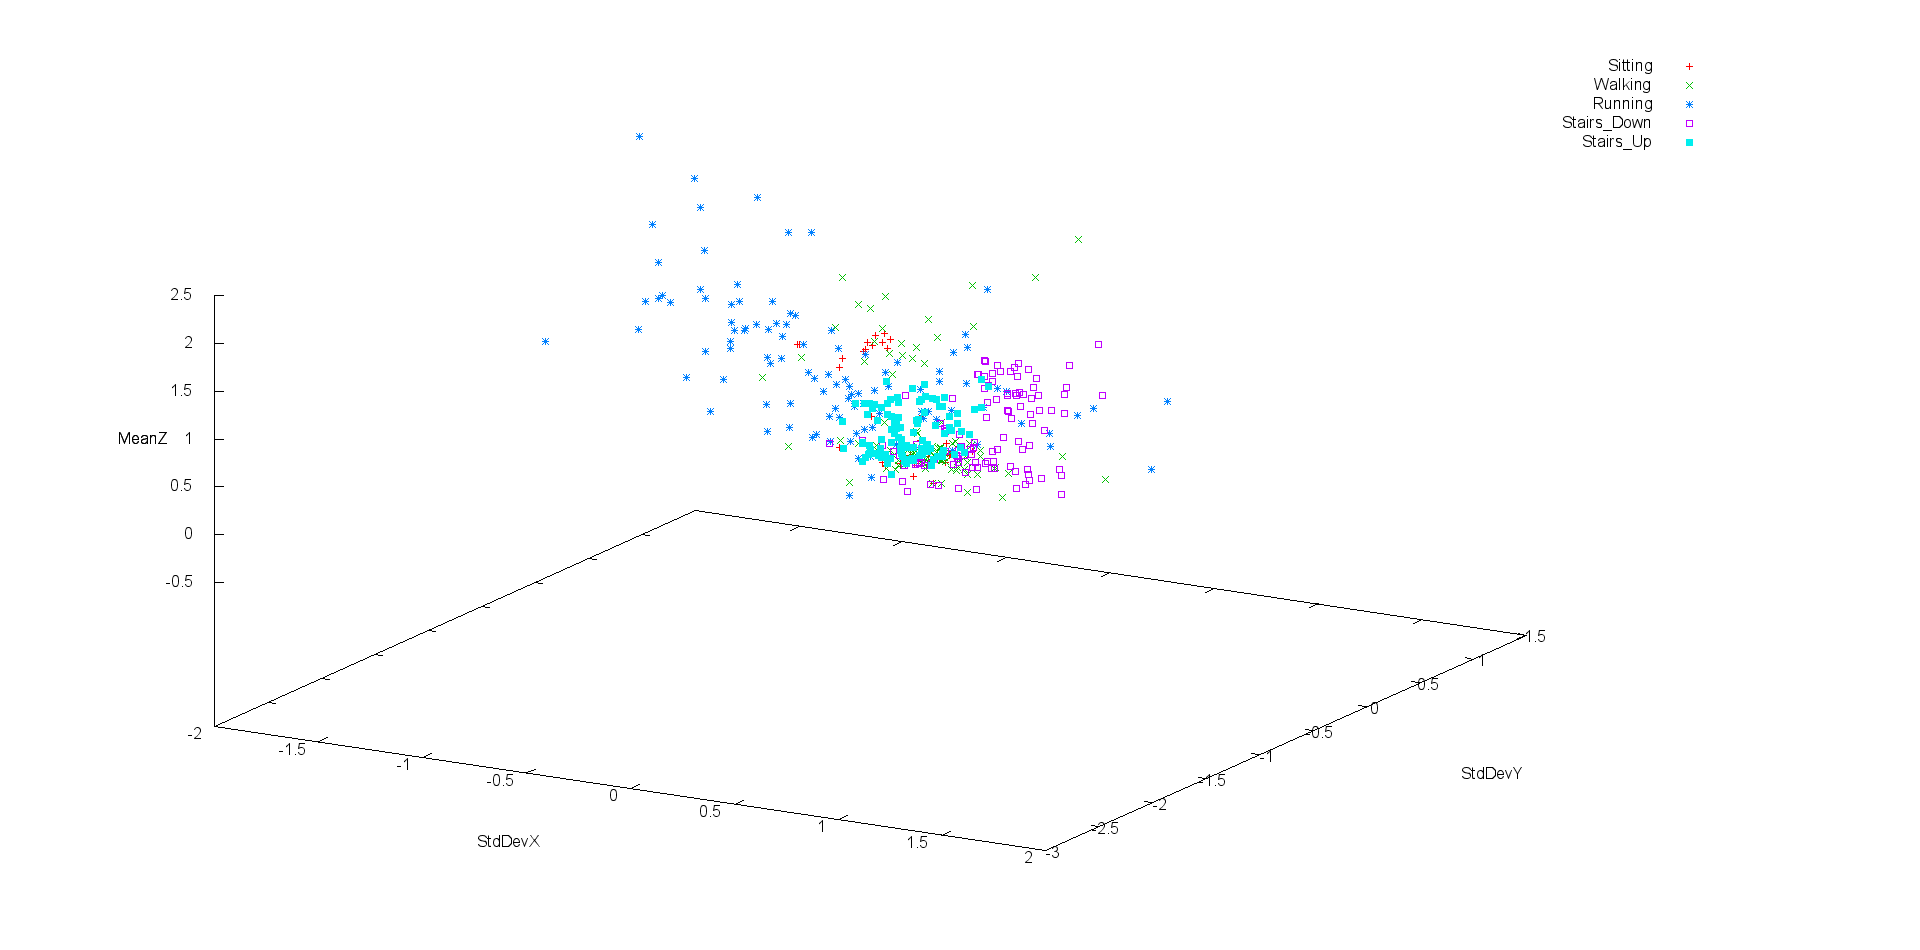
\includegraphics[width=0.9\textwidth]{../../data/training-plots/StdDev.png}
    \caption{Distribution of standard deviation in training set.}
    \label{fig:training-plot-stddev}
\end{figure}

\begin{figure}[ht]
    \centering
%    \begin{tikzpicture}[gnuplot]
%% generated with GNUPLOT 4.7p0 (Lua 5.1; terminal rev. 99, script rev. 100)
%% 6-5-2014 20:00:55
\path (0.000,0.000) rectangle (12.500,8.750);
\gpcolor{color=gp lt color border}
\gpsetlinetype{gp lt border}
\gpsetlinewidth{1.00}
\draw[gp path] (1.437,2.277)--(3.750,4.137);
\draw[gp path] (7.755,3.063)--(3.750,4.137);
\draw[gp path] (1.437,2.277)--(1.437,5.995);
\draw[gp path] (1.437,2.277)--(1.534,2.355);
\node[gp node center] at (1.338,2.144) {-2};
\draw[gp path] (3.750,4.137)--(3.653,4.059);
\draw[gp path] (1.938,2.143)--(2.035,2.221);
\node[gp node center] at (1.839,2.010) {-1.5};
\draw[gp path] (4.251,4.002)--(4.154,3.924);
\draw[gp path] (2.438,2.009)--(2.535,2.087);
\node[gp node center] at (2.339,1.875) {-1};
\draw[gp path] (4.750,3.868)--(4.653,3.790);
\draw[gp path] (2.939,1.875)--(3.036,1.953);
\node[gp node center] at (2.840,1.741) {-0.5};
\draw[gp path] (5.251,3.734)--(5.154,3.656);
\draw[gp path] (3.440,1.740)--(3.537,1.818);
\node[gp node center] at (3.341,1.607) { 0};
\draw[gp path] (5.752,3.600)--(5.655,3.522);
\draw[gp path] (3.941,1.606)--(4.038,1.684);
\node[gp node center] at (3.842,1.473) { 0.5};
\draw[gp path] (6.253,3.466)--(6.156,3.388);
\draw[gp path] (4.442,1.472)--(4.539,1.550);
\node[gp node center] at (4.342,1.339) { 1};
\draw[gp path] (6.754,3.331)--(6.657,3.254);
\draw[gp path] (4.941,1.338)--(5.038,1.416);
\node[gp node center] at (4.842,1.205) { 1.5};
\draw[gp path] (7.254,3.197)--(7.157,3.119);
\draw[gp path] (5.442,1.204)--(5.539,1.282);
\node[gp node center] at (5.343,1.070) { 2};
\draw[gp path] (7.755,3.063)--(7.658,2.985);
\draw[gp path] (5.442,1.204)--(5.286,1.245);
\node[gp node center] at (5.601,1.132) {-3};
\draw[gp path] (1.437,2.277)--(1.593,2.235);
\draw[gp path] (5.699,1.410)--(5.543,1.452);
\node[gp node center] at (5.858,1.339) {-2.5};
\draw[gp path] (1.694,2.484)--(1.850,2.442);
\draw[gp path] (5.956,1.617)--(5.800,1.659);
\node[gp node center] at (6.115,1.545) {-2};
\draw[gp path] (1.951,2.690)--(2.107,2.649);
\draw[gp path] (6.213,1.824)--(6.057,1.865);
\node[gp node center] at (6.372,1.752) {-1.5};
\draw[gp path] (2.208,2.897)--(2.364,2.855);
\draw[gp path] (6.470,2.030)--(6.314,2.072);
\node[gp node center] at (6.629,1.959) {-1};
\draw[gp path] (2.465,3.104)--(2.621,3.062);
\draw[gp path] (6.727,2.237)--(6.571,2.278);
\node[gp node center] at (6.886,2.165) {-0.5};
\draw[gp path] (2.722,3.310)--(2.878,3.268);
\draw[gp path] (6.984,2.443)--(6.828,2.485);
\node[gp node center] at (7.143,2.372) { 0};
\draw[gp path] (2.979,3.517)--(3.135,3.475);
\draw[gp path] (7.241,2.650)--(7.085,2.692);
\node[gp node center] at (7.400,2.578) { 0.5};
\draw[gp path] (3.236,3.723)--(3.392,3.682);
\draw[gp path] (7.498,2.856)--(7.342,2.898);
\node[gp node center] at (7.657,2.785) { 1};
\draw[gp path] (3.493,3.930)--(3.649,3.888);
\draw[gp path] (7.755,3.063)--(7.599,3.105);
\node[gp node center] at (7.914,2.992) { 1.5};
\draw[gp path] (3.750,4.137)--(3.906,4.095);
\draw[gp path] (1.437,3.517)--(1.617,3.517);
\node[gp node right] at (1.077,3.517) {-0.5};
\draw[gp path] (1.437,3.930)--(1.617,3.930);
\node[gp node right] at (1.077,3.930) { 0};
\draw[gp path] (1.437,4.343)--(1.617,4.343);
\node[gp node right] at (1.077,4.343) { 0.5};
\draw[gp path] (1.437,4.755)--(1.617,4.755);
\node[gp node right] at (1.077,4.755) { 1};
\draw[gp path] (1.437,5.169)--(1.617,5.169);
\node[gp node right] at (1.077,5.169) { 1.5};
\draw[gp path] (1.437,5.582)--(1.617,5.582);
\node[gp node right] at (1.077,5.582) { 2};
\draw[gp path] (1.437,5.995)--(1.617,5.995);
\node[gp node right] at (1.077,5.995) { 2.5};
\node[gp node center] at (0.149,4.755) {MeanZ};
\node[gp node right] at (10.143,7.645) {Sitting};
\gpcolor{color=gp lt color 0}
\gpsetpointsize{4.00}
\gppoint{gp mark 1}{(4.980,4.632)}
\gppoint{gp mark 1}{(4.980,4.633)}
\gppoint{gp mark 1}{(4.981,4.633)}
\gppoint{gp mark 1}{(4.981,4.633)}
\gppoint{gp mark 1}{(4.981,4.633)}
\gppoint{gp mark 1}{(4.980,4.633)}
\gppoint{gp mark 1}{(4.981,4.634)}
\gppoint{gp mark 1}{(4.980,4.633)}
\gppoint{gp mark 1}{(4.980,4.632)}
\gppoint{gp mark 1}{(4.980,4.633)}
\gppoint{gp mark 1}{(4.981,4.633)}
\gppoint{gp mark 1}{(4.980,4.633)}
\gppoint{gp mark 1}{(4.979,4.633)}
\gppoint{gp mark 1}{(4.879,4.607)}
\gppoint{gp mark 1}{(4.811,4.549)}
\gppoint{gp mark 1}{(4.901,4.372)}
\gppoint{gp mark 1}{(4.792,4.623)}
\gppoint{gp mark 1}{(4.765,4.590)}
\gppoint{gp mark 1}{(4.741,4.547)}
\gppoint{gp mark 1}{(4.778,4.684)}
\gppoint{gp mark 1}{(4.654,4.556)}
\gppoint{gp mark 1}{(4.848,4.961)}
\gppoint{gp mark 1}{(4.634,4.627)}
\gppoint{gp mark 1}{(4.668,4.513)}
\gppoint{gp mark 1}{(4.444,4.690)}
\gppoint{gp mark 1}{(4.604,4.952)}
\gppoint{gp mark 1}{(4.665,5.671)}
\gppoint{gp mark 1}{(4.621,5.652)}
\gppoint{gp mark 1}{(4.608,5.571)}
\gppoint{gp mark 1}{(4.694,5.618)}
\gppoint{gp mark 1}{(4.679,5.546)}
\gppoint{gp mark 1}{(4.655,5.592)}
\gppoint{gp mark 1}{(4.579,5.590)}
\gppoint{gp mark 1}{(4.561,5.514)}
\gppoint{gp mark 1}{(4.571,5.536)}
\gppoint{gp mark 1}{(4.460,5.454)}
\gppoint{gp mark 1}{(4.447,5.381)}
\gppoint{gp mark 1}{(4.253,5.575)}
\gppoint{gp mark 1}{(4.243,5.580)}
\gppoint{gp mark 1}{(4.981,4.632)}
\gppoint{gp mark 1}{(4.981,4.632)}
\gppoint{gp mark 1}{(4.982,4.632)}
\gppoint{gp mark 1}{(4.981,4.631)}
\gppoint{gp mark 1}{(4.982,4.632)}
\gppoint{gp mark 1}{(4.982,4.634)}
\gppoint{gp mark 1}{(4.981,4.634)}
\gppoint{gp mark 1}{(4.981,4.632)}
\gppoint{gp mark 1}{(4.981,4.632)}
\gppoint{gp mark 1}{(4.982,4.633)}
\gppoint{gp mark 1}{(4.981,4.632)}
\gppoint{gp mark 1}{(4.981,4.633)}
\gppoint{gp mark 1}{(4.982,4.633)}
\gppoint{gp mark 1}{(4.981,4.632)}
\gppoint{gp mark 1}{(4.982,4.633)}
\gppoint{gp mark 1}{(4.982,4.633)}
\gppoint{gp mark 1}{(4.981,4.634)}
\gppoint{gp mark 1}{(4.981,4.632)}
\gppoint{gp mark 1}{(4.981,4.632)}
\gppoint{gp mark 1}{(4.981,4.633)}
\gppoint{gp mark 1}{(4.981,4.632)}
\gppoint{gp mark 1}{(4.981,4.632)}
\gppoint{gp mark 1}{(4.981,4.634)}
\gppoint{gp mark 1}{(4.981,4.633)}
\gppoint{gp mark 1}{(4.982,4.634)}
\gppoint{gp mark 1}{(4.980,4.629)}
\gppoint{gp mark 1}{(4.980,4.625)}
\gppoint{gp mark 1}{(4.978,4.623)}
\gppoint{gp mark 1}{(4.979,4.623)}
\gppoint{gp mark 1}{(4.978,4.623)}
\gppoint{gp mark 1}{(4.979,4.623)}
\gppoint{gp mark 1}{(4.979,4.623)}
\gppoint{gp mark 1}{(4.978,4.623)}
\gppoint{gp mark 1}{(4.978,4.624)}
\gppoint{gp mark 1}{(4.979,4.623)}
\gppoint{gp mark 1}{(4.979,4.623)}
\gppoint{gp mark 1}{(4.979,4.623)}
\gppoint{gp mark 1}{(4.979,4.623)}
\gppoint{gp mark 1}{(4.980,4.623)}
\gppoint{gp mark 1}{(4.979,4.623)}
\gppoint{gp mark 1}{(4.978,4.624)}
\gppoint{gp mark 1}{(4.980,4.623)}
\gppoint{gp mark 1}{(4.979,4.623)}
\gppoint{gp mark 1}{(4.980,4.622)}
\gppoint{gp mark 1}{(4.965,4.726)}
\gppoint{gp mark 1}{(4.980,4.620)}
\gppoint{gp mark 1}{(4.980,4.620)}
\gppoint{gp mark 1}{(4.804,4.430)}
\gppoint{gp mark 1}{(4.957,4.555)}
\gppoint{gp mark 1}{(4.985,4.624)}
\gppoint{gp mark 1}{(4.839,4.749)}
\gppoint{gp mark 1}{(4.819,4.567)}
\gppoint{gp mark 1}{(5.024,4.700)}
\gppoint{gp mark 1}{(5.090,4.657)}
\gppoint{gp mark 1}{(4.981,4.632)}
\gppoint{gp mark 1}{(4.982,4.632)}
\gppoint{gp mark 1}{(4.982,4.633)}
\gppoint{gp mark 1}{(4.982,4.631)}
\gppoint{gp mark 1}{(4.982,4.631)}
\gppoint{gp mark 1}{(4.981,4.632)}
\gppoint{gp mark 1}{(4.982,4.632)}
\gppoint{gp mark 1}{(4.981,4.632)}
\gppoint{gp mark 1}{(4.981,4.632)}
\gppoint{gp mark 1}{(4.981,4.631)}
\gppoint{gp mark 1}{(4.982,4.632)}
\gppoint{gp mark 1}{(4.981,4.631)}
\gppoint{gp mark 1}{(4.981,4.631)}
\gppoint{gp mark 1}{(4.982,4.633)}
\gppoint{gp mark 1}{(4.982,4.632)}
\gppoint{gp mark 1}{(4.982,4.631)}
\gppoint{gp mark 1}{(4.981,4.633)}
\gppoint{gp mark 1}{(10.785,7.645)}
\gpcolor{color=gp lt color border}
\node[gp node right] at (10.143,7.337) {Walking};
\gpcolor{color=gp lt color 1}
\gppoint{gp mark 2}{(4.830,4.603)}
\gppoint{gp mark 2}{(4.923,4.678)}
\gppoint{gp mark 2}{(4.993,4.726)}
\gppoint{gp mark 2}{(4.842,4.564)}
\gppoint{gp mark 2}{(4.946,4.576)}
\gppoint{gp mark 2}{(4.898,4.372)}
\gppoint{gp mark 2}{(4.943,4.645)}
\gppoint{gp mark 2}{(4.759,4.559)}
\gppoint{gp mark 2}{(4.936,4.618)}
\gppoint{gp mark 2}{(4.821,4.825)}
\gppoint{gp mark 2}{(4.822,4.616)}
\gppoint{gp mark 2}{(4.933,4.684)}
\gppoint{gp mark 2}{(4.735,4.524)}
\gppoint{gp mark 2}{(4.762,4.632)}
\gppoint{gp mark 2}{(4.914,4.646)}
\gppoint{gp mark 2}{(4.716,4.494)}
\gppoint{gp mark 2}{(4.772,4.556)}
\gppoint{gp mark 2}{(4.738,4.692)}
\gppoint{gp mark 2}{(4.938,4.588)}
\gppoint{gp mark 2}{(4.815,4.652)}
\gppoint{gp mark 2}{(4.867,4.669)}
\gppoint{gp mark 2}{(4.821,4.678)}
\gppoint{gp mark 2}{(4.846,4.659)}
\gppoint{gp mark 2}{(4.759,4.625)}
\gppoint{gp mark 2}{(4.804,4.607)}
\gppoint{gp mark 2}{(4.734,4.577)}
\gppoint{gp mark 2}{(4.853,4.561)}
\gppoint{gp mark 2}{(4.925,4.587)}
\gppoint{gp mark 2}{(4.803,4.683)}
\gppoint{gp mark 2}{(4.827,4.586)}
\gppoint{gp mark 2}{(4.696,4.662)}
\gppoint{gp mark 2}{(4.707,4.623)}
\gppoint{gp mark 2}{(4.674,4.501)}
\gppoint{gp mark 2}{(4.494,4.383)}
\gppoint{gp mark 2}{(4.938,4.907)}
\gppoint{gp mark 2}{(4.841,4.597)}
\gppoint{gp mark 2}{(4.776,4.662)}
\gppoint{gp mark 2}{(4.779,4.580)}
\gppoint{gp mark 2}{(4.753,4.701)}
\gppoint{gp mark 2}{(4.756,4.526)}
\gppoint{gp mark 2}{(5.393,6.150)}
\gppoint{gp mark 2}{(5.096,5.734)}
\gppoint{gp mark 2}{(4.825,4.805)}
\gppoint{gp mark 2}{(4.630,4.666)}
\gppoint{gp mark 2}{(4.877,5.789)}
\gppoint{gp mark 2}{(4.667,4.904)}
\gppoint{gp mark 2}{(4.534,4.722)}
\gppoint{gp mark 2}{(4.752,5.485)}
\gppoint{gp mark 2}{(4.857,5.409)}
\gppoint{gp mark 2}{(5.087,6.087)}
\gppoint{gp mark 2}{(4.800,5.453)}
\gppoint{gp mark 2}{(4.818,5.551)}
\gppoint{gp mark 2}{(4.705,5.321)}
\gppoint{gp mark 2}{(4.627,4.708)}
\gppoint{gp mark 2}{(4.920,5.634)}
\gppoint{gp mark 2}{(4.687,5.499)}
\gppoint{gp mark 2}{(4.449,4.750)}
\gppoint{gp mark 2}{(4.747,5.581)}
\gppoint{gp mark 2}{(4.596,5.886)}
\gppoint{gp mark 2}{(4.617,5.605)}
\gppoint{gp mark 2}{(4.669,5.994)}
\gppoint{gp mark 2}{(4.658,5.717)}
\gppoint{gp mark 2}{(4.564,5.430)}
\gppoint{gp mark 2}{(4.197,4.699)}
\gppoint{gp mark 2}{(4.536,5.922)}
\gppoint{gp mark 2}{(4.462,6.154)}
\gppoint{gp mark 2}{(4.426,5.726)}
\gppoint{gp mark 2}{(4.263,5.467)}
\gppoint{gp mark 2}{(4.076,5.295)}
\gppoint{gp mark 2}{(4.895,4.694)}
\gppoint{gp mark 2}{(4.990,4.494)}
\gppoint{gp mark 2}{(4.794,4.642)}
\gppoint{gp mark 2}{(4.879,4.561)}
\gppoint{gp mark 2}{(4.902,4.623)}
\gppoint{gp mark 2}{(4.889,4.557)}
\gppoint{gp mark 2}{(4.956,4.605)}
\gppoint{gp mark 2}{(4.870,4.604)}
\gppoint{gp mark 2}{(4.905,4.620)}
\gppoint{gp mark 2}{(4.942,4.576)}
\gppoint{gp mark 2}{(4.882,4.557)}
\gppoint{gp mark 2}{(5.010,4.485)}
\gppoint{gp mark 2}{(4.934,4.678)}
\gppoint{gp mark 2}{(5.018,4.505)}
\gppoint{gp mark 2}{(4.863,4.497)}
\gppoint{gp mark 2}{(5.600,6.484)}
\gppoint{gp mark 2}{(5.084,4.706)}
\gppoint{gp mark 2}{(5.050,4.492)}
\gppoint{gp mark 2}{(4.831,4.546)}
\gppoint{gp mark 2}{(5.125,4.613)}
\gppoint{gp mark 2}{(5.129,4.664)}
\gppoint{gp mark 2}{(4.960,4.568)}
\gppoint{gp mark 2}{(5.009,4.740)}
\gppoint{gp mark 2}{(4.793,4.700)}
\gppoint{gp mark 2}{(4.949,4.606)}
\gppoint{gp mark 2}{(5.076,4.721)}
\gppoint{gp mark 2}{(4.982,4.638)}
\gppoint{gp mark 2}{(5.065,4.558)}
\gppoint{gp mark 2}{(5.057,4.614)}
\gppoint{gp mark 2}{(5.023,4.570)}
\gppoint{gp mark 2}{(5.195,4.503)}
\gppoint{gp mark 2}{(5.198,4.509)}
\gppoint{gp mark 2}{(5.111,4.444)}
\gppoint{gp mark 2}{(5.063,4.448)}
\gppoint{gp mark 2}{(4.941,4.369)}
\gppoint{gp mark 2}{(5.233,4.249)}
\gppoint{gp mark 2}{(5.065,4.290)}
\gppoint{gp mark 2}{(5.260,4.458)}
\gppoint{gp mark 2}{(5.520,4.614)}
\gppoint{gp mark 2}{(5.727,4.401)}
\gppoint{gp mark 2}{(4.853,4.550)}
\gppoint{gp mark 2}{(10.785,7.337)}
\gpcolor{color=gp lt color border}
\node[gp node right] at (10.143,7.029) {Running};
\gpcolor{color=gp lt color 2}
\gppoint{gp mark 3}{(4.683,5.211)}
\gppoint{gp mark 3}{(4.639,4.978)}
\gppoint{gp mark 3}{(4.606,4.857)}
\gppoint{gp mark 3}{(4.537,5.152)}
\gppoint{gp mark 3}{(4.491,5.211)}
\gppoint{gp mark 3}{(4.491,5.211)}
\gppoint{gp mark 3}{(4.599,4.614)}
\gppoint{gp mark 3}{(4.445,4.943)}
\gppoint{gp mark 3}{(4.538,4.590)}
\gppoint{gp mark 3}{(4.843,4.999)}
\gppoint{gp mark 3}{(4.368,5.172)}
\gppoint{gp mark 3}{(4.618,5.176)}
\gppoint{gp mark 3}{(4.558,5.064)}
\gppoint{gp mark 3}{(4.516,5.043)}
\gppoint{gp mark 3}{(4.208,5.071)}
\gppoint{gp mark 3}{(4.564,4.839)}
\gppoint{gp mark 3}{(5.058,5.236)}
\gppoint{gp mark 3}{(4.475,5.270)}
\gppoint{gp mark 3}{(4.392,5.317)}
\gppoint{gp mark 3}{(4.496,4.740)}
\gppoint{gp mark 3}{(4.046,5.752)}
\gppoint{gp mark 3}{(4.442,5.541)}
\gppoint{gp mark 3}{(4.525,4.805)}
\gppoint{gp mark 3}{(4.572,5.493)}
\gppoint{gp mark 3}{(4.424,5.027)}
\gppoint{gp mark 3}{(4.336,4.804)}
\gppoint{gp mark 3}{(4.401,4.740)}
\gppoint{gp mark 3}{(4.317,4.772)}
\gppoint{gp mark 3}{(3.939,5.695)}
\gppoint{gp mark 3}{(4.395,4.958)}
\gppoint{gp mark 3}{(4.271,5.572)}
\gppoint{gp mark 3}{(4.875,4.996)}
\gppoint{gp mark 3}{(3.990,5.711)}
\gppoint{gp mark 3}{(4.206,4.860)}
\gppoint{gp mark 3}{(4.429,5.230)}
\gppoint{gp mark 3}{(3.632,5.942)}
\gppoint{gp mark 3}{(4.190,5.750)}
\gppoint{gp mark 3}{(4.486,5.114)}
\gppoint{gp mark 3}{(4.486,5.114)}
\gppoint{gp mark 3}{(4.092,5.060)}
\gppoint{gp mark 3}{(3.823,5.000)}
\gppoint{gp mark 3}{(3.593,6.001)}
\gppoint{gp mark 3}{(4.322,5.287)}
\gppoint{gp mark 3}{(3.511,5.949)}
\gppoint{gp mark 3}{(4.111,5.409)}
\gppoint{gp mark 3}{(4.100,5.463)}
\gppoint{gp mark 3}{(4.165,5.456)}
\gppoint{gp mark 3}{(3.886,5.276)}
\gppoint{gp mark 3}{(3.919,5.606)}
\gppoint{gp mark 3}{(3.479,5.705)}
\gppoint{gp mark 3}{(4.503,5.145)}
\gppoint{gp mark 3}{(3.711,5.289)}
\gppoint{gp mark 3}{(4.098,4.828)}
\gppoint{gp mark 3}{(4.297,5.331)}
\gppoint{gp mark 3}{(3.027,5.602)}
\gppoint{gp mark 3}{(4.123,5.949)}
\gppoint{gp mark 3}{(4.406,5.699)}
\gppoint{gp mark 3}{(4.168,5.645)}
\gppoint{gp mark 3}{(4.210,5.844)}
\gppoint{gp mark 3}{(4.103,5.708)}
\gppoint{gp mark 3}{(4.141,5.754)}
\gppoint{gp mark 3}{(4.232,5.829)}
\gppoint{gp mark 3}{(3.921,5.540)}
\gppoint{gp mark 3}{(4.202,6.546)}
\gppoint{gp mark 3}{(3.986,5.699)}
\gppoint{gp mark 3}{(4.309,6.538)}
\gppoint{gp mark 3}{(3.962,5.945)}
\gppoint{gp mark 3}{(3.954,6.092)}
\gppoint{gp mark 3}{(3.926,5.924)}
\gppoint{gp mark 3}{(3.802,5.520)}
\gppoint{gp mark 3}{(3.927,5.769)}
\gppoint{gp mark 3}{(3.798,5.970)}
\gppoint{gp mark 3}{(4.049,6.841)}
\gppoint{gp mark 3}{(3.571,5.976)}
\gppoint{gp mark 3}{(3.775,6.755)}
\gppoint{gp mark 3}{(3.572,6.280)}
\gppoint{gp mark 3}{(3.777,6.052)}
\gppoint{gp mark 3}{(3.793,6.389)}
\gppoint{gp mark 3}{(3.545,6.608)}
\gppoint{gp mark 3}{(3.745,7.010)}
\gppoint{gp mark 3}{(3.482,7.372)}
\gppoint{gp mark 3}{(4.672,5.337)}
\gppoint{gp mark 3}{(4.853,4.656)}
\gppoint{gp mark 3}{(4.854,4.935)}
\gppoint{gp mark 3}{(5.254,5.167)}
\gppoint{gp mark 3}{(4.604,4.422)}
\gppoint{gp mark 3}{(4.722,4.711)}
\gppoint{gp mark 3}{(4.931,5.345)}
\gppoint{gp mark 3}{(5.114,4.715)}
\gppoint{gp mark 3}{(4.987,5.009)}
\gppoint{gp mark 3}{(4.914,4.927)}
\gppoint{gp mark 3}{(4.990,4.665)}
\gppoint{gp mark 3}{(4.931,5.261)}
\gppoint{gp mark 3}{(5.056,5.658)}
\gppoint{gp mark 3}{(4.931,5.261)}
\gppoint{gp mark 3}{(4.838,5.190)}
\gppoint{gp mark 3}{(6.027,5.086)}
\gppoint{gp mark 3}{(5.063,5.553)}
\gppoint{gp mark 3}{(4.999,5.505)}
\gppoint{gp mark 3}{(5.161,6.054)}
\gppoint{gp mark 3}{(4.730,5.418)}
\gppoint{gp mark 3}{(5.141,5.033)}
\gppoint{gp mark 3}{(4.494,4.269)}
\gppoint{gp mark 3}{(5.465,4.696)}
\gppoint{gp mark 3}{(5.325,4.896)}
\gppoint{gp mark 3}{(5.211,5.194)}
\gppoint{gp mark 3}{(5.461,4.807)}
\gppoint{gp mark 3}{(5.670,5.023)}
\gppoint{gp mark 3}{(5.594,4.964)}
\gppoint{gp mark 3}{(5.949,4.488)}
\gppoint{gp mark 3}{(10.785,7.029)}
\gpcolor{color=gp lt color border}
\node[gp node right] at (10.143,6.721) {Stairs_Down};
\gpcolor{color=gp lt color 3}
\gppoint{gp mark 4}{(4.858,4.526)}
\gppoint{gp mark 4}{(5.185,5.257)}
\gppoint{gp mark 4}{(5.274,5.342)}
\gppoint{gp mark 4}{(5.147,5.194)}
\gppoint{gp mark 4}{(5.150,5.428)}
\gppoint{gp mark 4}{(4.955,4.855)}
\gppoint{gp mark 4}{(4.936,4.894)}
\gppoint{gp mark 4}{(4.961,4.828)}
\gppoint{gp mark 4}{(4.661,4.401)}
\gppoint{gp mark 4}{(5.120,5.315)}
\gppoint{gp mark 4}{(5.159,5.076)}
\gppoint{gp mark 4}{(5.115,5.320)}
\gppoint{gp mark 4}{(5.147,5.296)}
\gppoint{gp mark 4}{(4.711,4.656)}
\gppoint{gp mark 4}{(4.993,5.110)}
\gppoint{gp mark 4}{(5.148,5.436)}
\gppoint{gp mark 4}{(4.846,4.556)}
\gppoint{gp mark 4}{(4.556,4.751)}
\gppoint{gp mark 4}{(4.765,5.139)}
\gppoint{gp mark 4}{(4.658,4.707)}
\gppoint{gp mark 4}{(4.395,4.725)}
\gppoint{gp mark 4}{(5.184,5.323)}
\gppoint{gp mark 4}{(4.835,4.554)}
\gppoint{gp mark 4}{(5.158,4.944)}
\gppoint{gp mark 4}{(5.211,5.392)}
\gppoint{gp mark 4}{(5.166,5.225)}
\gppoint{gp mark 4}{(4.739,4.615)}
\gppoint{gp mark 4}{(5.095,4.684)}
\gppoint{gp mark 4}{(5.291,5.381)}
\gppoint{gp mark 4}{(5.311,5.413)}
\gppoint{gp mark 4}{(5.015,4.595)}
\gppoint{gp mark 4}{(5.036,4.699)}
\gppoint{gp mark 4}{(5.224,5.342)}
\gppoint{gp mark 4}{(4.815,4.538)}
\gppoint{gp mark 4}{(5.258,5.003)}
\gppoint{gp mark 4}{(4.822,4.710)}
\gppoint{gp mark 4}{(4.908,4.581)}
\gppoint{gp mark 4}{(5.012,4.619)}
\gppoint{gp mark 4}{(5.256,5.157)}
\gppoint{gp mark 4}{(5.152,4.547)}
\gppoint{gp mark 4}{(5.203,5.101)}
\gppoint{gp mark 4}{(5.238,4.770)}
\gppoint{gp mark 4}{(4.751,4.391)}
\gppoint{gp mark 4}{(4.763,4.532)}
\gppoint{gp mark 4}{(4.814,4.562)}
\gppoint{gp mark 4}{(5.336,5.147)}
\gppoint{gp mark 4}{(5.295,5.150)}
\gppoint{gp mark 4}{(5.260,4.995)}
\gppoint{gp mark 4}{(5.304,5.300)}
\gppoint{gp mark 4}{(4.997,4.540)}
\gppoint{gp mark 4}{(4.964,4.835)}
\gppoint{gp mark 4}{(5.398,5.283)}
\gppoint{gp mark 4}{(5.100,4.731)}
\gppoint{gp mark 4}{(4.891,4.554)}
\gppoint{gp mark 4}{(5.404,5.139)}
\gppoint{gp mark 4}{(5.258,5.135)}
\gppoint{gp mark 4}{(5.082,4.624)}
\gppoint{gp mark 4}{(4.888,4.363)}
\gppoint{gp mark 4}{(5.209,4.669)}
\gppoint{gp mark 4}{(5.375,5.112)}
\gppoint{gp mark 4}{(5.275,4.941)}
\gppoint{gp mark 4}{(5.410,5.003)}
\gppoint{gp mark 4}{(5.050,4.620)}
\gppoint{gp mark 4}{(5.380,5.204)}
\gppoint{gp mark 4}{(5.358,5.358)}
\gppoint{gp mark 4}{(5.366,4.970)}
\gppoint{gp mark 4}{(5.023,4.327)}
\gppoint{gp mark 4}{(5.321,5.038)}
\gppoint{gp mark 4}{(4.776,4.300)}
\gppoint{gp mark 4}{(4.961,4.657)}
\gppoint{gp mark 4}{(5.302,5.140)}
\gppoint{gp mark 4}{(4.925,4.354)}
\gppoint{gp mark 4}{(5.025,4.803)}
\gppoint{gp mark 4}{(5.554,5.397)}
\gppoint{gp mark 4}{(5.020,4.660)}
\gppoint{gp mark 4}{(5.379,4.896)}
\gppoint{gp mark 4}{(5.317,5.159)}
\gppoint{gp mark 4}{(5.539,5.208)}
\gppoint{gp mark 4}{(5.021,4.559)}
\gppoint{gp mark 4}{(5.189,4.568)}
\gppoint{gp mark 4}{(5.163,4.563)}
\gppoint{gp mark 4}{(5.533,5.144)}
\gppoint{gp mark 4}{(5.312,4.737)}
\gppoint{gp mark 4}{(5.101,4.558)}
\gppoint{gp mark 4}{(5.471,5.006)}
\gppoint{gp mark 4}{(5.113,4.505)}
\gppoint{gp mark 4}{(5.185,4.656)}
\gppoint{gp mark 4}{(5.055,4.463)}
\gppoint{gp mark 4}{(5.180,4.499)}
\gppoint{gp mark 4}{(5.091,4.511)}
\gppoint{gp mark 4}{(5.109,4.319)}
\gppoint{gp mark 4}{(5.294,4.476)}
\gppoint{gp mark 4}{(5.693,5.574)}
\gppoint{gp mark 4}{(5.530,4.978)}
\gppoint{gp mark 4}{(5.078,4.669)}
\gppoint{gp mark 4}{(5.433,4.834)}
\gppoint{gp mark 4}{(5.715,5.138)}
\gppoint{gp mark 4}{(5.363,4.703)}
\gppoint{gp mark 4}{(5.272,4.519)}
\gppoint{gp mark 4}{(5.327,4.668)}
\gppoint{gp mark 4}{(5.197,4.503)}
\gppoint{gp mark 4}{(5.300,4.327)}
\gppoint{gp mark 4}{(5.354,4.490)}
\gppoint{gp mark 4}{(5.364,4.393)}
\gppoint{gp mark 4}{(5.510,4.494)}
\gppoint{gp mark 4}{(5.345,4.363)}
\gppoint{gp mark 4}{(5.361,4.448)}
\gppoint{gp mark 4}{(5.516,4.439)}
\gppoint{gp mark 4}{(5.421,4.411)}
\gppoint{gp mark 4}{(5.518,4.272)}
\gppoint{gp mark 4}{(10.785,6.721)}
\gpcolor{color=gp lt color border}
\node[gp node right] at (10.143,6.413) {Stairs_Up};
\gpcolor{color=gp lt color 4}
\gppoint{gp mark 5}{(5.166,5.213)}
\gppoint{gp mark 5}{(4.846,4.681)}
\gppoint{gp mark 5}{(5.098,5.018)}
\gppoint{gp mark 5}{(4.802,4.597)}
\gppoint{gp mark 5}{(5.134,5.274)}
\gppoint{gp mark 5}{(5.001,4.630)}
\gppoint{gp mark 5}{(5.015,4.896)}
\gppoint{gp mark 5}{(5.134,5.034)}
\gppoint{gp mark 5}{(5.017,4.980)}
\gppoint{gp mark 5}{(4.847,4.646)}
\gppoint{gp mark 5}{(4.747,4.727)}
\gppoint{gp mark 5}{(4.752,4.614)}
\gppoint{gp mark 5}{(4.976,4.864)}
\gppoint{gp mark 5}{(5.038,4.830)}
\gppoint{gp mark 5}{(4.979,4.956)}
\gppoint{gp mark 5}{(4.769,4.550)}
\gppoint{gp mark 5}{(4.885,4.676)}
\gppoint{gp mark 5}{(4.989,4.838)}
\gppoint{gp mark 5}{(4.956,4.810)}
\gppoint{gp mark 5}{(4.873,4.655)}
\gppoint{gp mark 5}{(4.745,4.640)}
\gppoint{gp mark 5}{(4.912,4.876)}
\gppoint{gp mark 5}{(4.805,4.691)}
\gppoint{gp mark 5}{(4.867,4.710)}
\gppoint{gp mark 5}{(4.748,4.757)}
\gppoint{gp mark 5}{(4.785,4.584)}
\gppoint{gp mark 5}{(4.873,4.714)}
\gppoint{gp mark 5}{(4.745,4.702)}
\gppoint{gp mark 5}{(4.947,5.039)}
\gppoint{gp mark 5}{(4.772,4.705)}
\gppoint{gp mark 5}{(4.843,5.102)}
\gppoint{gp mark 5}{(4.733,4.777)}
\gppoint{gp mark 5}{(4.928,5.039)}
\gppoint{gp mark 5}{(4.836,4.619)}
\gppoint{gp mark 5}{(4.822,4.896)}
\gppoint{gp mark 5}{(4.777,4.689)}
\gppoint{gp mark 5}{(4.671,4.626)}
\gppoint{gp mark 5}{(4.914,5.104)}
\gppoint{gp mark 5}{(4.846,4.628)}
\gppoint{gp mark 5}{(4.859,5.234)}
\gppoint{gp mark 5}{(4.859,4.990)}
\gppoint{gp mark 5}{(4.645,4.683)}
\gppoint{gp mark 5}{(4.862,5.124)}
\gppoint{gp mark 5}{(4.741,4.665)}
\gppoint{gp mark 5}{(4.692,4.595)}
\gppoint{gp mark 5}{(4.650,4.761)}
\gppoint{gp mark 5}{(4.679,4.549)}
\gppoint{gp mark 5}{(4.582,4.627)}
\gppoint{gp mark 5}{(4.955,5.116)}
\gppoint{gp mark 5}{(4.714,4.811)}
\gppoint{gp mark 5}{(4.649,4.602)}
\gppoint{gp mark 5}{(4.667,4.621)}
\gppoint{gp mark 5}{(4.819,4.922)}
\gppoint{gp mark 5}{(4.894,5.107)}
\gppoint{gp mark 5}{(4.697,4.445)}
\gppoint{gp mark 5}{(4.831,4.930)}
\gppoint{gp mark 5}{(4.801,5.197)}
\gppoint{gp mark 5}{(4.662,4.600)}
\gppoint{gp mark 5}{(4.700,4.735)}
\gppoint{gp mark 5}{(4.618,4.637)}
\gppoint{gp mark 5}{(4.805,4.819)}
\gppoint{gp mark 5}{(4.807,4.580)}
\gppoint{gp mark 5}{(4.646,4.665)}
\gppoint{gp mark 5}{(4.638,4.619)}
\gppoint{gp mark 5}{(4.741,4.862)}
\gppoint{gp mark 5}{(4.587,4.707)}
\gppoint{gp mark 5}{(4.592,4.635)}
\gppoint{gp mark 5}{(4.834,5.088)}
\gppoint{gp mark 5}{(4.722,4.909)}
\gppoint{gp mark 5}{(4.600,4.666)}
\gppoint{gp mark 5}{(4.555,4.727)}
\gppoint{gp mark 5}{(4.733,4.948)}
\gppoint{gp mark 5}{(4.761,4.565)}
\gppoint{gp mark 5}{(4.556,4.567)}
\gppoint{gp mark 5}{(4.722,4.855)}
\gppoint{gp mark 5}{(4.741,4.681)}
\gppoint{gp mark 5}{(4.730,4.945)}
\gppoint{gp mark 5}{(4.701,4.844)}
\gppoint{gp mark 5}{(4.464,4.683)}
\gppoint{gp mark 5}{(4.696,5.106)}
\gppoint{gp mark 5}{(4.760,4.703)}
\gppoint{gp mark 5}{(4.572,4.598)}
\gppoint{gp mark 5}{(4.734,5.075)}
\gppoint{gp mark 5}{(4.714,4.930)}
\gppoint{gp mark 5}{(4.556,4.720)}
\gppoint{gp mark 5}{(4.713,4.905)}
\gppoint{gp mark 5}{(4.630,4.924)}
\gppoint{gp mark 5}{(4.619,5.059)}
\gppoint{gp mark 5}{(4.697,4.952)}
\gppoint{gp mark 5}{(4.682,5.065)}
\gppoint{gp mark 5}{(4.649,5.035)}
\gppoint{gp mark 5}{(4.680,4.969)}
\gppoint{gp mark 5}{(4.729,5.115)}
\gppoint{gp mark 5}{(4.565,5.069)}
\gppoint{gp mark 5}{(4.607,5.028)}
\gppoint{gp mark 5}{(4.461,4.915)}
\gppoint{gp mark 5}{(4.590,5.071)}
\gppoint{gp mark 5}{(4.580,4.975)}
\gppoint{gp mark 5}{(4.675,5.255)}
\gppoint{gp mark 5}{(4.521,5.071)}
\gppoint{gp mark 5}{(4.893,4.525)}
\gppoint{gp mark 5}{(4.901,4.586)}
\gppoint{gp mark 5}{(4.921,4.612)}
\gppoint{gp mark 5}{(4.947,4.608)}
\gppoint{gp mark 5}{(4.949,4.660)}
\gppoint{gp mark 5}{(4.947,4.640)}
\gppoint{gp mark 5}{(4.849,4.751)}
\gppoint{gp mark 5}{(5.033,4.690)}
\gppoint{gp mark 5}{(5.076,4.798)}
\gppoint{gp mark 5}{(5.052,4.649)}
\gppoint{gp mark 5}{(10.785,6.413)}
\gpcolor{color=gp lt color border}
\draw[gp path] (7.755,3.063)--(5.442,1.204);
\draw[gp path] (1.437,2.277)--(5.442,1.204);
\node[gp node center] at (2.862,1.276) {MeanX};
\node[gp node center] at (7.600,1.865) {MeanY};
\node[gp node center] at (0.149,4.755) {MeanZ};
%% coordinates of the plot area
\gpdefrectangularnode{gp plot 1}{\pgfpoint{1.437cm}{0.771cm}}{\pgfpoint{7.755cm}{8.287cm}}
\end{tikzpicture}
%% gnuplot variables

    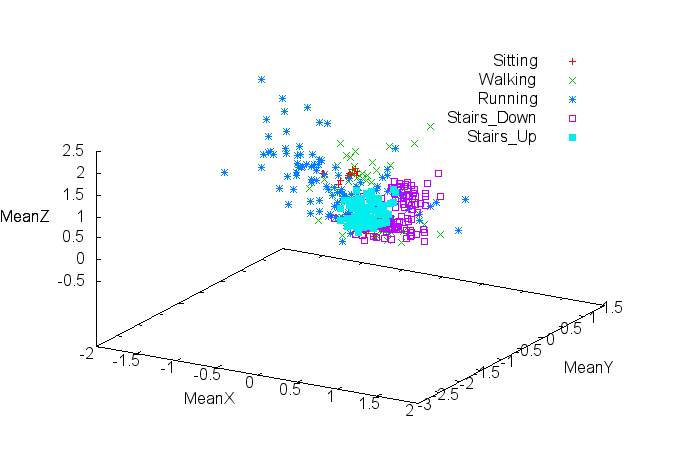
\includegraphics[width=0.9\textwidth]{../../data/training-plots/Means.png}
    \caption{Distribution of the means in training set.}
    \label{fig:training-plot-means}
\end{figure}

\begin{figure}[ht]
    \centering
    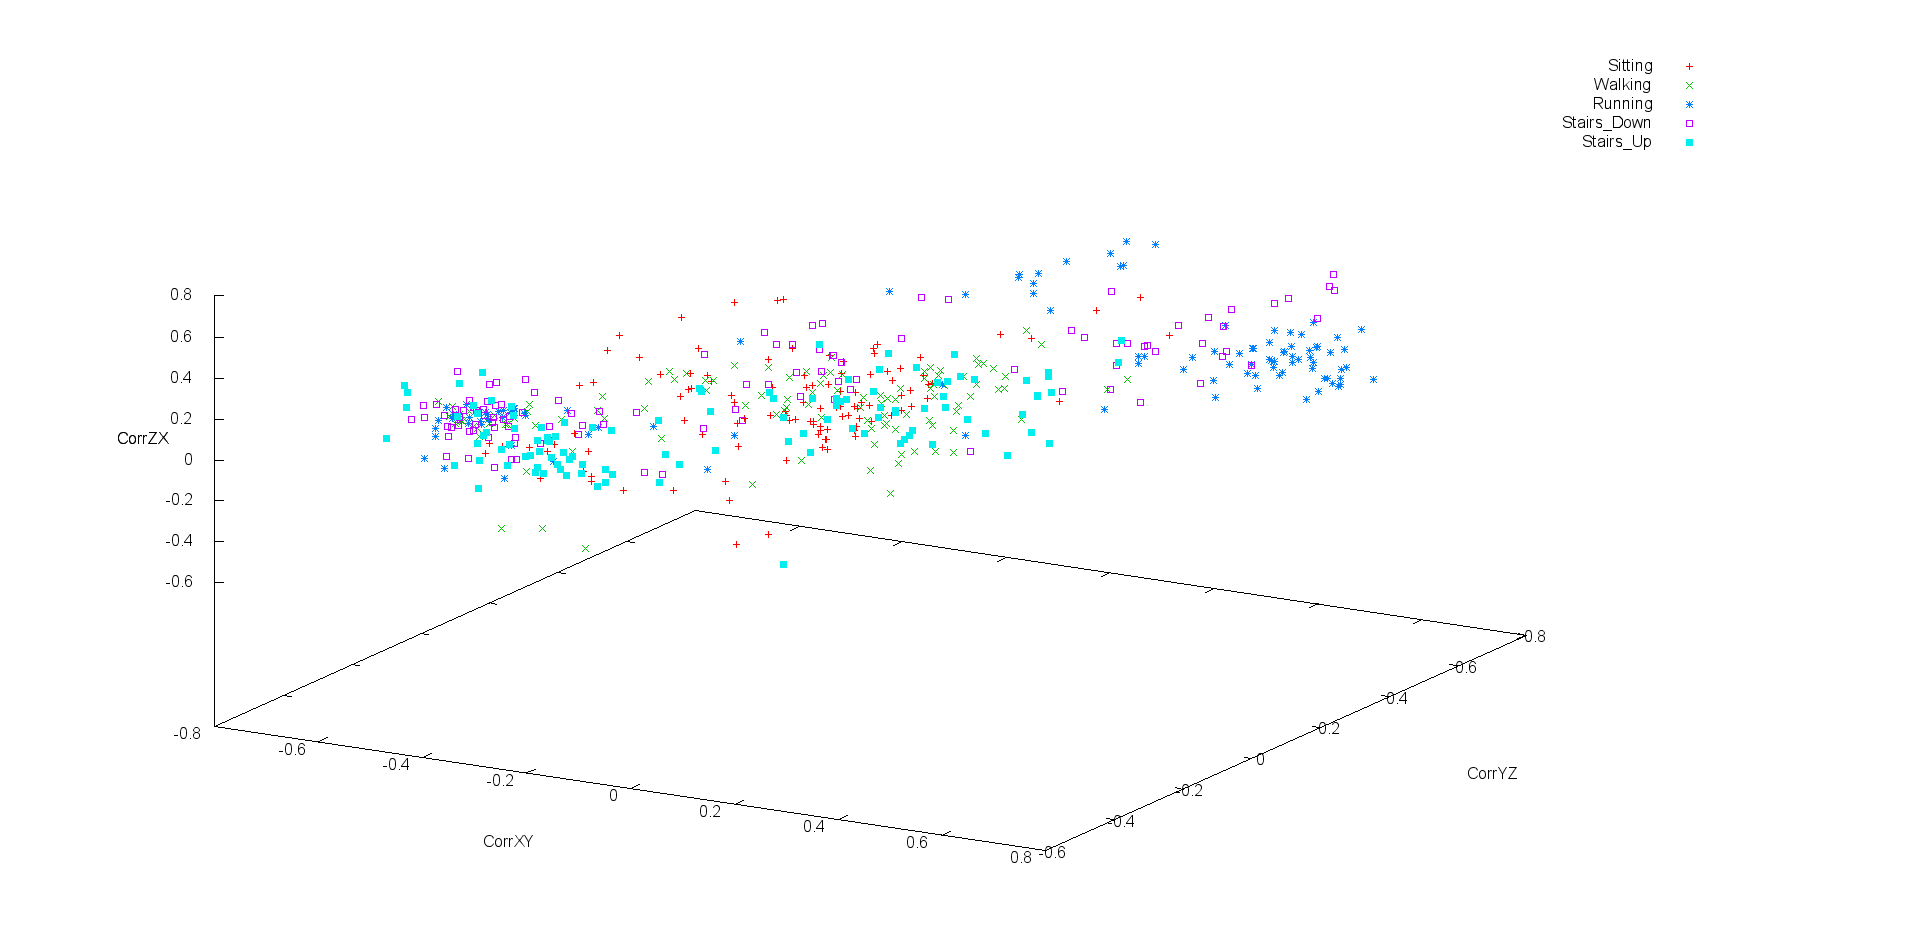
\includegraphics[width=0.9\textwidth]{../../data/training-plots/Corr.png}
    \caption{Distribution of the correlation in training set.}
    \label{fig:training-plot-corr}
\end{figure}

\begin{figure}[ht]
    \centering
    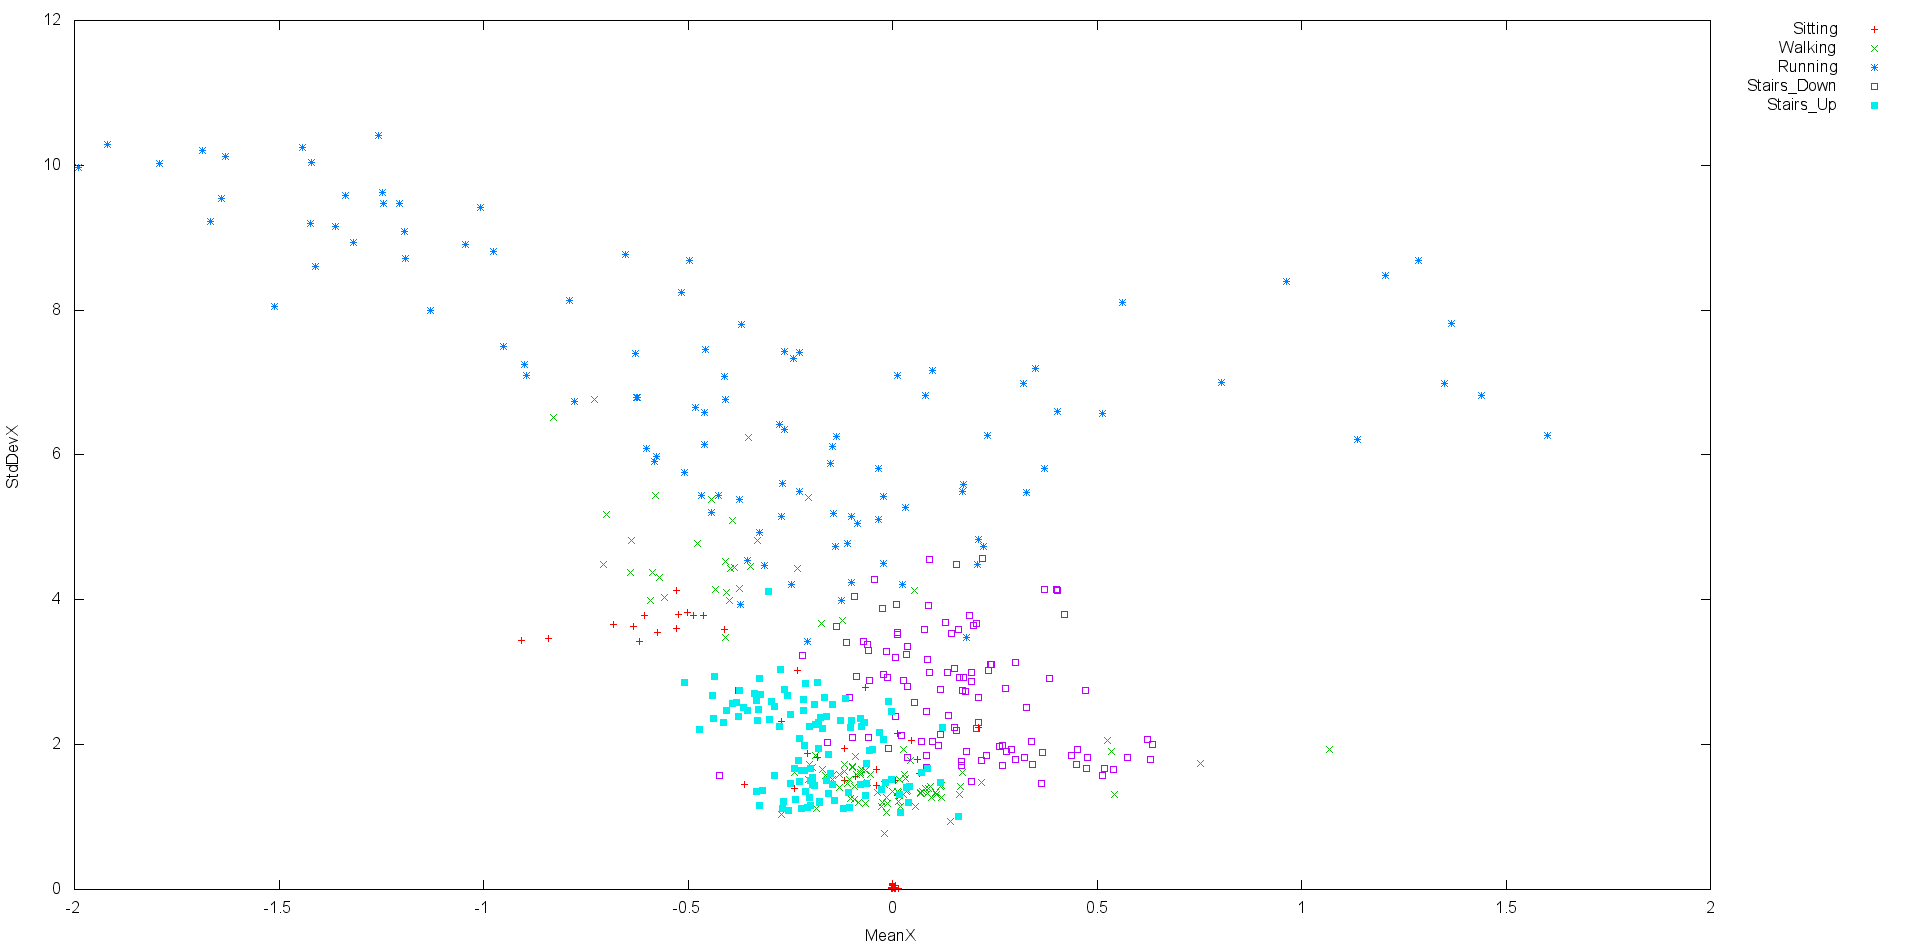
\includegraphics[width=0.9\textwidth]{../../data/training-plots/X.png}
    \caption{Standard deviation and mean of x-axis.}
    \label{fig:training-plot-x}
\end{figure}

\begin{figure}[ht]
    \centering
    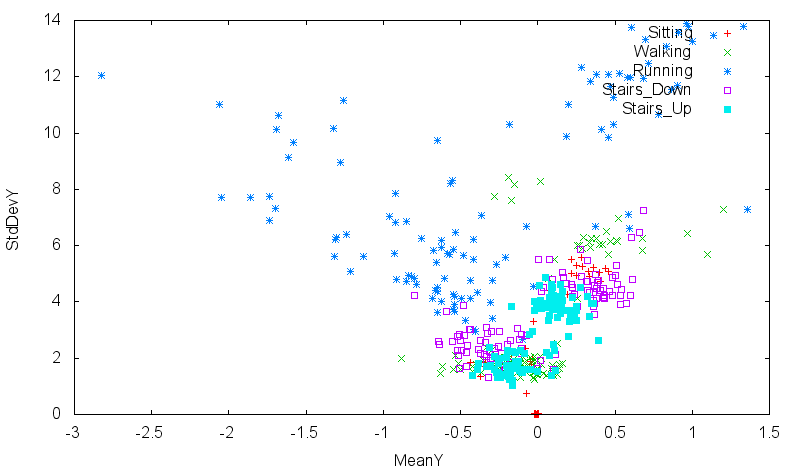
\includegraphics[width=0.9\textwidth]{../../data/training-plots/Y.png}
    \caption{Standard deviation and mean of y-axis.}
    \label{fig:training-plot-y}
\end{figure}

\begin{figure}[ht]
    \centering
    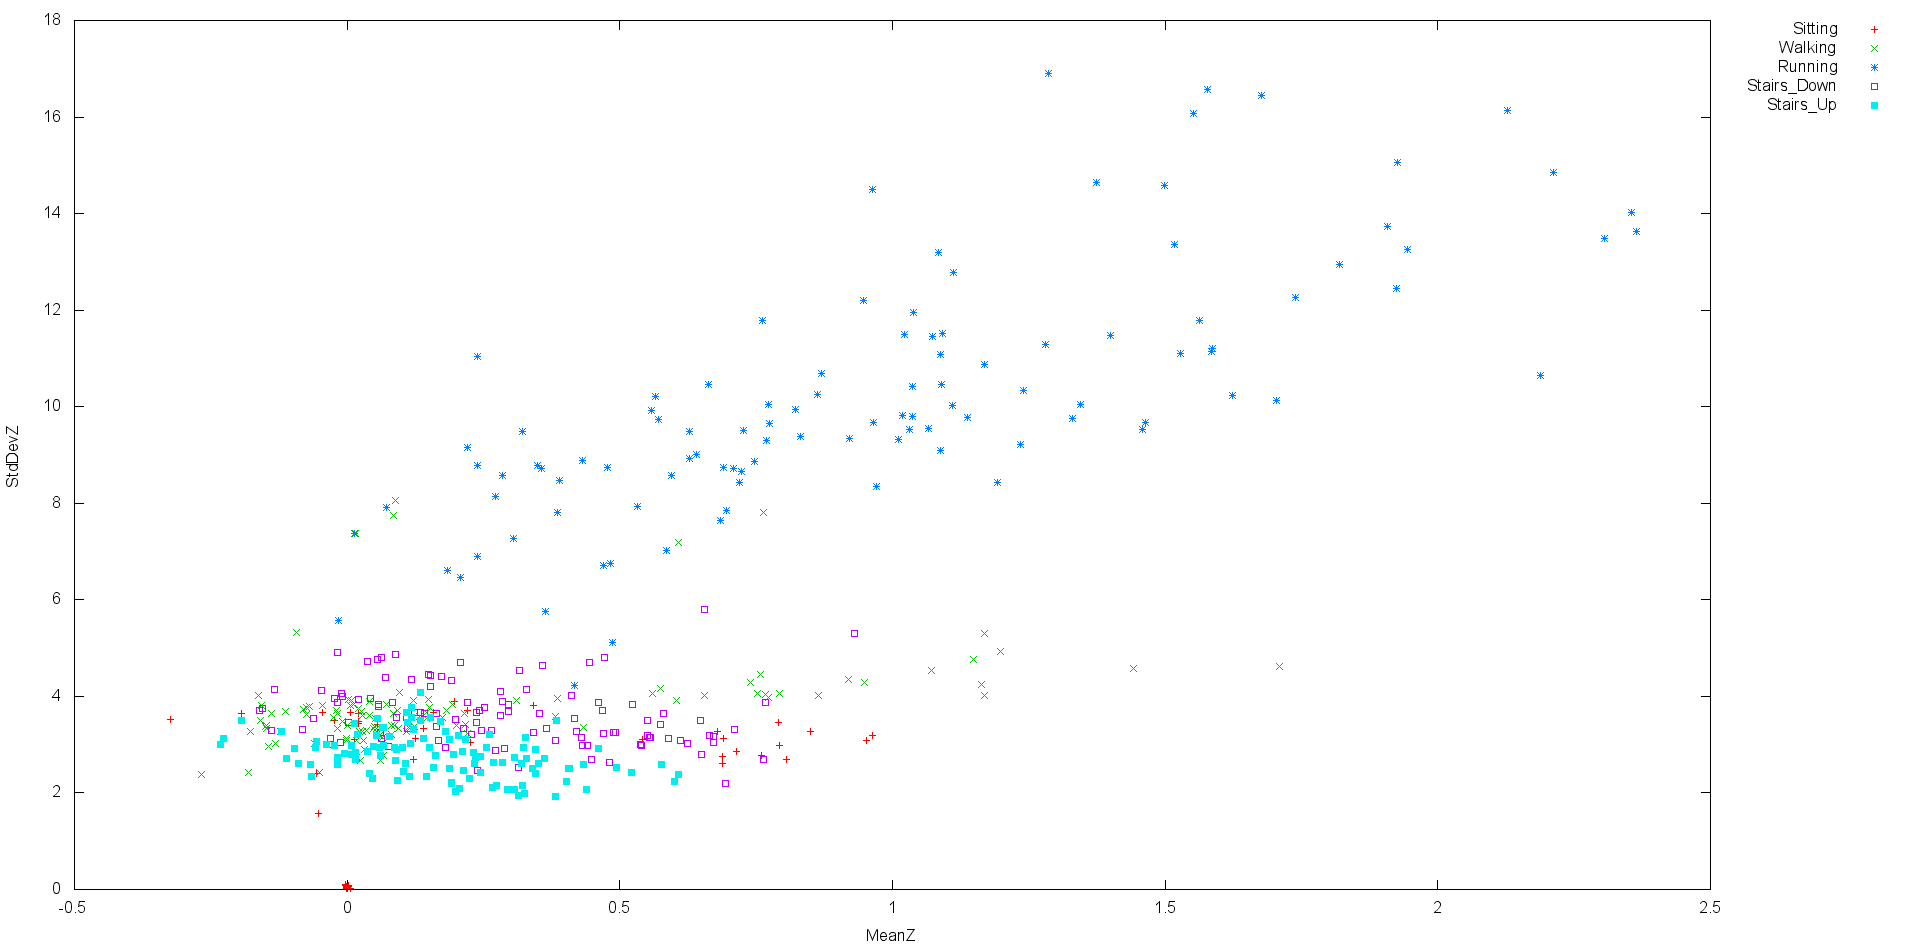
\includegraphics[width=0.9\textwidth]{../../data/training-plots/Z.png}
    \caption{Standard deviation and mean of z-axis.}
    \label{fig:training-plot-z}
\end{figure}


\end{document}
